% update 17/04/2026
\documentclass[journal]{IEEEtran}
\usepackage{cite}
\usepackage{amsmath,amsfonts,amssymb}
\usepackage{graphicx,caption}
\usepackage{epstopdf}
\usepackage{subcaption}
\usepackage{url}
\usepackage{color}
\usepackage{colortbl}
\usepackage{multirow}
\usepackage{bm}
\usepackage{algorithm}
\usepackage{algpseudocode}
\usepackage{booktabs}
\usepackage[table,xcdraw]{xcolor}
\usepackage{booktabs}
\usepackage{tabularx}
\usepackage{array}
\newcolumntype{L}{>{\raggedright\arraybackslash}X}

\newcommand{\SNR}{\mathsf{SNR}}
\newcommand{\INR}{\mathsf{INR}}
\newcommand{\E}{\mathbb{E}}
\newcommand{\Var}{\mathrm{Var}}
\newcommand{\Cov}{\mathrm{Cov}}
\newcommand{\sym}{\mathrm{sym}}
\newcommand{\conv}{\mathrm{conv}}
\newcommand{\jg}{\mathrm{J.G.}}
\newcommand{\rank}{\mathrm{rank}}
\newcommand{\Id}{\mathbf{I}}
\newcommand{\Zero}{\mathbf{0}}
\newcommand{\figref}[1]{Fig.~\ref{#1}}
\newcommand{\tabref}[1]{Table~\ref{#1}}

\title{Pose Estimation and EDLines Algorithm Based Virtual Encoder for XY Axis Calibration of a 3-Axis 3D Printer}

\author{
Zayd Zihni Zaidan,~\IEEEmembership{Member,~IEEE},
Sylmina Dalily Alkaff,
Aqilah Baseri Huddin,
Hanim Hussin,
Asif Ali Zamzami,~\IEEEmembership{Member,~IEEE}
and Bahrudin
%
\thanks{Manuscript received xxx; revised xxx; accepted xxx. Date of publication xxx; date of current version xxx. (\textit{Corresponding author: Asif Ali Zamzami.})}
%
\thanks{Zayd Zihni Zaidan, Sylmina Dalily Alkaff, and Asif Ali Zamzami are with the Department of Robotics and Artificial Intelligence Engineering, Faculty of Advanced Technology and Multidiscipline, Universitas Airlangga, Surabaya 60115, Indonesia (e-mail: zayd.zihni.zaidan-2022@ftmm.unair.ac.id; sylmina.dalily.a@ftmm.unair.ac.id; asif.ali@ftmm.unair.ac.id).}
%
\thanks{Aqilah Baseri Huddin is with the Department of Electrical, Electronic and Systems Engineering, Faculty of Engineering and Built Environment, Universiti Kebangsaan Malaysia, Bangi 43600, Selangor, Malaysia (e-mail: aqilah@ukm.edu.my).}
%
\thanks{Hanim Hussin is with the Faculty of Electrical Engineering, Universiti Teknologi MARA, 40450 Shah Alam, Selangor, Malaysia (e-mail: hanimh@uitm.edu.my).}

\thanks{Bahrudin is with the Biomechatronics Research Group, Research Center for Intelligent Mechatronics, National Research and Innovation Agency (BRIN), Indonesia. (e-mail: bahr03@brin.go.id).}
}

\begin{document}
\maketitle

\begin{abstract}
In the era of Industry 4.0, virtual manufacturing paradigms are increasingly leveraged to optimize manual production and inspection processes. For desktop 3D printers, calibration shifts caused by mechanical wear over extended operating periods introduce severe geometric inaccuracies. Traditional calibration approaches rely heavily on mechanical dial gauges, which are inherently limited by human error, restricted dimensionality, and low time efficiency. Although automated alternatives have been proposed, they frequently encounter trade-offs between cost and spatial accuracy. To overcome these limitations, this study presents a highly accurate, precise, and cost-effective machine vision-based virtual encoder system designed for XY-axis calibration. The system incorporates a custom chessboard marker, a sub-pixel corner detection pipeline utilizing the Edge Drawing Lines (EDLines) algorithm, and a Levenberg-Marquardt-driven Perspective-n-Point (SolvePnP) solver to dynamically convert camera pixel displacements into micrometer-scale physical positions. The system enables comprehensive error profiling and real-time compensation for axis steps per millimeter, structural backlash, and axis skewness. Experimental validation recorded an internal measurement error below 7~$\mu$m ($3.55~\mu$m for the X-axis and $6.25~\mu$m for the Y-axis), operating under a maximum environmental noise threshold of 4.9~$\mu$m. Linear axis calibration yielded post-compensation errors within 5.4--7.1~$\mu$m, representing an accuracy enhancement of 84.6\% and 90.2\% for the X and Y axes, respectively. Furthermore, simultaneous tracking evaluations along complex eliptic test trajectories demonstrated a 54.24\% reduction in total tracking error, decreasing the root-mean-square error (RMSE) from 100.9~$\mu$m to 46.17~$\mu$m. The system successfully mitigated baseline trajectory deviations by more than half, establishing the virtual encoder as a highly viable, low-cost ($<$ 30 USD) alternative for precision desktop metrology.
\end{abstract}

\begin{IEEEkeywords}
Virtual Encoder, Machine Vision, 3D Printer Calibration, Edge Drawing Lines, Chessboard Marker.
\end{IEEEkeywords}

\IEEEpeerreviewmaketitle

% --- INCLUSION SECTION MATTERS ---
\section{Introduction}
\IEEEPARstart{T}{he} advancement of Industry 4.0 has introduced a new paradigm in the manufacturing sector through the seamless integration of physical and digital systems \cite{soori2024}. A key concept emerging from this transformation is virtual manufacturing, a production approach that integrates sensor data, digital models, and intelligent devices to achieve real-time process optimization \cite{soori2024}. Within the context of modern manufacturing, virtual inspection and quality control systems play a critical role\cite{soori2024}. These systems leverage imaging technology and visual data processing to monitor, analyze, and guarantee product quality without direct physical intervention \cite{soori2024}. In material extrusion systems like 3D printers, apart from chemical and thermal extrusion parameters, the absolute positioning accuracy of the machine's mechanical movements significantly influences the quality of the printed model \cite{zaborniak2024}. With prolonged utilization, the pulley and belt linear motion transmission systems can undergo calibration drift due to structural relaxation and mechanical wear \cite{xu2020, zaborniak2024, papageorgiou2019}. Traditional calibration methods for high-precision machinery employ a mechanical dial gauge for error profiling by evaluating the deviation between the actual displacement and the commanded position \cite{iso230_1_2012}. Despite offering a fine measurement resolution down to 10~$\mu$m, this manual approach suffers from several drawbacks, including susceptibility to human error and poor time efficiency.

Several prior studies have developed automated calibration methods using physical sensors for 3D printers; however, such hardware automation incurs a significant cost increase. Examples of research attempting to automate error profiling and 3D printer calibration include inductive methods \cite{Schouten2022}, camera-based systems using Hue Saturation Value (HSV) color segmentation algorithms \cite{Chen2025}, laser triangulation \cite{Munteanu2021}, and computer vision integrated with planar ArUco markers \cite{Owais2026}. From an implementation cost perspective, the computer vision approach combined with ArUco represents the most cost-effective solution, as it only requires a standard camera and paper-printed markers. Nevertheless, this method falls short in terms of accuracy, exhibiting a measurement tolerance error of 84~$\mu$m. This accuracy level is inferior to that of the inductive method, which achieves a translational accuracy of 45~$\mu$m with a repeatability of 2~$\mu$m \cite{Schouten2022}. Hence, there is an urgent need to develop an automated kinematic calibration approach for desktop 3D printers that is highly accurate, precise, and cost-effective.

To address this need, this study proposes the concept of a virtual encoder system that adopts the fundamental principles of marker-based position tracking, leveraging computer vision and fiducial markers. The virtual encoder is designed to translate camera pixel shifts into actual machine displacements, effectively substituting the function of a physical rotary encoder. By employing this system, machine parameters such as steps per millimeter, alongside geometric and kinematic errors like backlash and skewness, can be evaluated by analyzing the positional deviations along the machine axes captured by the camera. The resulting error profiling data is subsequently utilized to execute error compensation during machine calibration. This study focuses primarily on XY-axis calibration, as Z-axis alignment can already be reliably achieved using electromechanical limit switches or inductive proximity sensors \cite{Schouten2022}.
\section{System Architecture and Marker Selection Rationale}
\label{rationale}
Although it shares the same underlying concept as the previous study \cite{Owais2026}, this method is further refined to achieve a significantly higher sub-pixel precision level by replacing the ArUco fiducial marker with a chessboard marker. Based on its geometric characteristics, the chessboard marker offers vastly superior performance for sub-pixel corner detection requirements compared to ArUco \cite{Triyono2024, Dan2022}. Through sub-pixel corner detection using algorithms such as EDLines (Edge Drawing Lines), the chessboard marker can yield a highly precise average reprojection error ranging from 0.044 to 0.05 pixels \cite{Dan2022}. On the other hand, while ArUco's primary advantage lies in its functionality as a unique identifier that is highly robust against environmental noise, its spatial corner detection sharpness does not match the clear line intersections of a chessboard marker. 

As a hybrid solution, the ChArUco algorithm is frequently deployed because it combines the geometric sharpness of a chessboard with the robust identification of ArUco to handle visual occlusion and extreme environmental conditions, achieving a pose detection success rate of 97.4\cite{Hu2019}. However, a ChArUco implementation is considered overkill within the scope of this study, as its unique code identification feature becomes redundant in an ideal, controlled 3D printer workspace that is free from occlusion issues. 

The accurate corner detection results obtained from this chessboard are subsequently utilized in the pose estimation process to secure precise positional readouts. In this study, the algorithm selected for pose estimation is the Iterative SolvePnP (Perspective-n-Point) \cite{opencv_solvepnp}. The selection of the Iterative SolvePnP algorithm—the default type in OpenCV—is based on its performance, which is deemed sufficient for pose estimation when coupled with a 3D model featuring highly accurate structural features like a chessboard \cite{Zhou2025}. In summary, a precise corner detection approach yields a sharper pose estimation accuracy compared to using standard ArUco markers. Through this approach, the measurement error in kinematic tracking is expected to be suppressed to a level significantly lower than that of the prior study, establishing a calibration solution that not only rivals the accuracy of industrial optical instruments but also incurs an exceptionally low implementation cost.
\section{Proposed Machine Vision-Based Virtual Encoder System}
\label{proposed_encoder}
The proposed virtual encoder operates by mapping sub-pixel visual coordinate transformations into physical metric positions. The core pipeline consists of raw image feature extraction, sub-pixel corner optimization, localized enhancement for homography alignment, pinhole model restoration, and iterative pose estimation.

\subsection{Sub-Pixel Feature Extraction Pipeline}
To preserve native intensity gradient sharpness ($\nabla I$) and avoid spatial boundary shifts, the sub-pixel feature extraction pipeline operates directly on the unenhanced raw grayscale image ($I_{\text{gray}}$). Applying contrast amplification or smoothing filter passes at this initial stage introduces spatial bias and blur artifacts that degrade sub-pixel corner accuracy.

First, the Edge Drawing Lines (EDLines) detector traces continuous pixel chains representing the structural border segments of the chessboard marker on $I_{\text{gray}}$. The line screening process evaluates edge junction topologies to filter background clutter, identifying line clusters intersecting at 3-way or 4-way junctions based on line lengths ($l$), boundary intersection radii ($r$), and angular deviation thresholds ($\theta$). Coarse pixel-level coordinates are initially generated using a localized least-squares line-fitting operator:

\begin{equation}
p = \min_{q_i \in N(p)} \sum \left( g_{q_i}^{\top} (q_i - p) \right)^2
\end{equation}

where $g_{q_i}$ represents the gray gradient vector at an adjacent neighborhood pixel $q_i$ centered around the corner estimation index $p$. Sub-pixel refinement is mathematically resolved by minimizing the projection error where the vector connecting the true corner to neighborhood structures is perfectly orthogonal to the local gradient, expressed analytically as:

\begin{equation}
p = \left(\sum_{q_i \in N(p)} g_{q_i} g_{q_i}^{\mathsf{T}}\right)^{-1} \cdot \sum_{q_i \in N(p)} \left(g_{q_i} g_{q_i}^{\mathsf{T}}\right) q_i
\end{equation}

%%%%%%%


\subsection{Homography Alignment and Corner Sorting}
To arrange the 49 extracted sub-pixel corners into a unified coordinate grid, three asymmetric internal circular elements located at the marker's center serve as spatial anchors. Unlike the sub-pixel optimization phase, anchor detection requires high local contrast and noise suppression to prevent false circle candidates. Therefore, image enhancement is selectively applied strictly within this sorting phase.

The grayscale image is first enhanced using Contrast Limited Adaptive Histogram Equalization (CLAHE) to amplify local contrast boundaries around the central anchor patterns. To suppress high-frequency noise and amplification artifacts induced by CLAHE, a 2D Gaussian blur convolves the enhanced image using a symmetric $5 \times 5$ kernel:

\begin{equation}
G_2(x,y) = \frac{1}{2\pi\sigma^2} e^{-\frac{x^2+y^2}{2\sigma^2}}
\end{equation}

where $\sigma$ acts as the standard deviation controlling the smoothing threshold. Isolating CLAHE and Gaussian filtering to this alignment stage enables robust anchor extraction via the Hough Gradient Circle Transform (or EDCircles) without corrupting the native pixel gradients used in sub-pixel corner optimization.

Following anchor centroid isolation, candidate corners are filtered to select the central $7 \times 7$ grid points. A homography transformation matrix $H$ is calculated using the four extreme boundary corners to project perspective coordinates into a structured $7 \times 7$ planar layout, effectively neutralizing out-of-plane rotation drifts and ordering corners in row-major sequence.

\subsection{Projection Mapping and Iterative SolvePnP}
The physical tracking domain relies on standard pinhole camera geometry. A 3D spatial coordinate vector $[X, Y, Z]^T$ defined in the world frame is projected onto the 2D image plane pixel index $[u, v, 1]^T$ via the intrinsic matrix ($K$) and extrinsic transformation profile ($[R|T]$):

\begin{equation}
s \begin{bmatrix} u \\ v \\ 1 \end{bmatrix} = \begin{bmatrix} f_x & 0 & c_x \\ 0 & f_y & c_y \\ 0 & 0 & 1 \end{bmatrix} \begin{bmatrix} R_{11} & R_{12} & R_{13} & T_x \\ R_{21} & R_{22} & R_{23} & T_y \\ R_{31} & R_{32} & R_{33} & T_z \end{bmatrix} \begin{bmatrix} X \\ Y \\ Z \\ 1 \end{bmatrix}
\end{equation}

where $s$ scales the perspective mapping, $f_x, f_y$ represent directional focal lengths, and $c_x, c_y$ pinpoint the sensor's principal optical center. Lens distortion is mitigated using an all-encompassing radial and tangential mapping law:

\begin{equation}
\begin{cases} 
x' = x(1 + k_1r^2 + k_2r^4) + 2p_1xy + p_2(r^2 + 2x^2) \\ 
y' = y(1 + k_1r^2 + k_2r^4) + p_1(r^2 + 2y^2) + 2p_2xy 
\end{cases}
\end{equation}

with $r^2 = x^2 + y^2$, mapping structural sensor anomalies through coefficients $k_n$ and $p_n$. 

The actual translation vector $T = [T_x, T_y, T_z]^T$ provides direct millimeter-scale metric tracking data, eliminating external scale factors. Finding the optimal camera pose is framed as a non-linear optimization problem solved using the iterative Levenberg-Marquardt (LM) method. The update vector ($\Delta x$) is updated at each step by adjusting a trust-region damping parameter ($u$):

\begin{equation}
\Delta x = (G^T G + uI)^{-1} G^T f(x)
\end{equation}

where $G$ denotes the calculated Jacobian matrix of the projection functions and $I$ defines a standard identity matrix.
\section{Mathematical Preliminaries and Problem Formulation}
\label{problem}
To conceptualize the virtual encoder system, the kinematic inaccuracies of a Cartesian XZ-head/Y-bed architecture must be mathematically modeled. Machine tool calibration requires the extraction and compensation of three primary error components: linear step drift, mechanical backlash, and structural axis skewness. 

\subsection{Linear Step Derivation}
The theoretical linear motion resolution of a pulley-and-belt mechanism is dictated by the motor's step angle, microstepping configurations, and the physical parameters of the transmission components \cite{M92}. The nominal configuration governs the steps executed per millimeter ($Steps/mm_{default}$) via the following analytical relation:

\begin{equation}
Steps/mm = \frac{\theta_{rev} \times M_f}{P_b \times N_g}
\end{equation}

where $\theta_{rev}$ is the physical steps per full motor revolution (typically 200 steps for a $1.8^\circ$ stepper motor), $M_f$ is the electronic microstepping factor applied by the driver, $P_b$ represents the belt pitch (e.g., 2~mm for standard GT2 profiles), and $N_g$ denotes the tooth count of the drive pulley. Mechanical degradation and wear alter this theoretical framework over time, creating a discrepancy between commanded distances ($D_{cmd}$) and physical displacements ($D_{act}$). The rectified steps per millimeter profile ($Steps/mm_{new}$) is computed via a proportional scale matching law:

\begin{equation}
Steps/mm_{new} = \left(\frac{D_{cmd}}{D_{act}}\right) \times Steps/mm_{old}
\end{equation}

\subsection{Backlash Modeling}
Mechanical backlash manifests as a nonlinear deadzone error when an axis undergoes a reversal of motion direction. The lost motion arises from physical clearances between meshing transmission components (e.g., belt-pulley slack) \cite{papageorgiou2019}. Mathematically, if $x_{in}(t)$ represents the commanded actuator position and $x_{out}(t)$ defines the actual joint coordinate, the structural deadzone is formulated as:

\begin{equation}
x_{out}(t) = 
\begin{cases} 
x_{in}(t) - d_b & \text{if } \dot{x}_{in}(t) > 0 \\
x_{in}(t) + d_b & \text{if } \dot{x}_{in}(t) < 0 
\end{cases}
\end{equation}

where $d_b$ represents the absolute backlash width. The virtual encoder quantifies this phenomenon by monitoring positional states across a predefined bi-directional travel sequence, evaluating the absolute divergence between the original anchor coordinate and the coordinates achieved post-reversal.

\subsection{Axis Skewness Formulation}
Structural misalignment during assembly or asymmetric belt tensioning destroys the strict orthogonality between the X and Y movement vectors ($\vec{V}_x$ and $\vec{V}_y$). The non-orthogonality angle ($\theta_{skew}$) represents the deviation of the internal angle ($\theta_{int}$) from an ideal $90^\circ$ perpendicular intersection. Let the absolute orientation angles ($\theta_{abs}$) of the motion vectors relative to a common reference plane be computed via the quadrant-corrected arctangent function:

\begin{equation}
\theta_{abs} = \arctan\left(\frac{y_n}{x_n}\right)
\end{equation}

The internal axis angle is extracted from the difference between the absolute angles of the vectors, allowing the dimensionless geometric correction factor ($I_{skew}$) to be isolated as follows:
\begin{equation}
I_{skew} = \tan(\theta_{skew}) = \tan(90^{\circ} - \theta_{int})
\end{equation}

where $x_n$ and $y_n$ are the measured position coordinates along the respective axes. $I_{skew}$ specifies the cross-talk adjustment or parasitic drift per unit displacement required to implement linear software pre-compensation.
\section{Experimental Methodology}
\label{methodology}
\subsection{System Setup}
In this study, the target machine is a Creality CR-10 V3 3D printer featuring an XZ-head architecture, while the visual sensor for the virtual encoder system is an OV9821 camera module operating at a resolution of $1280 \times 720$ pixels at 120 frames per second. To interface the camera with the machine, a custom PLA camera mount is employed. The camera is mounted directly on the X-carriage width with a fixed height of 260 mm from the print bed. The camera is placed to capture the displacement of a chessboard marker affixed to the Y-axis print bed. The visualization of the system setup is illustrated in \figref{fig:setup}. 

\begin{figure}[ht]
    \centering
    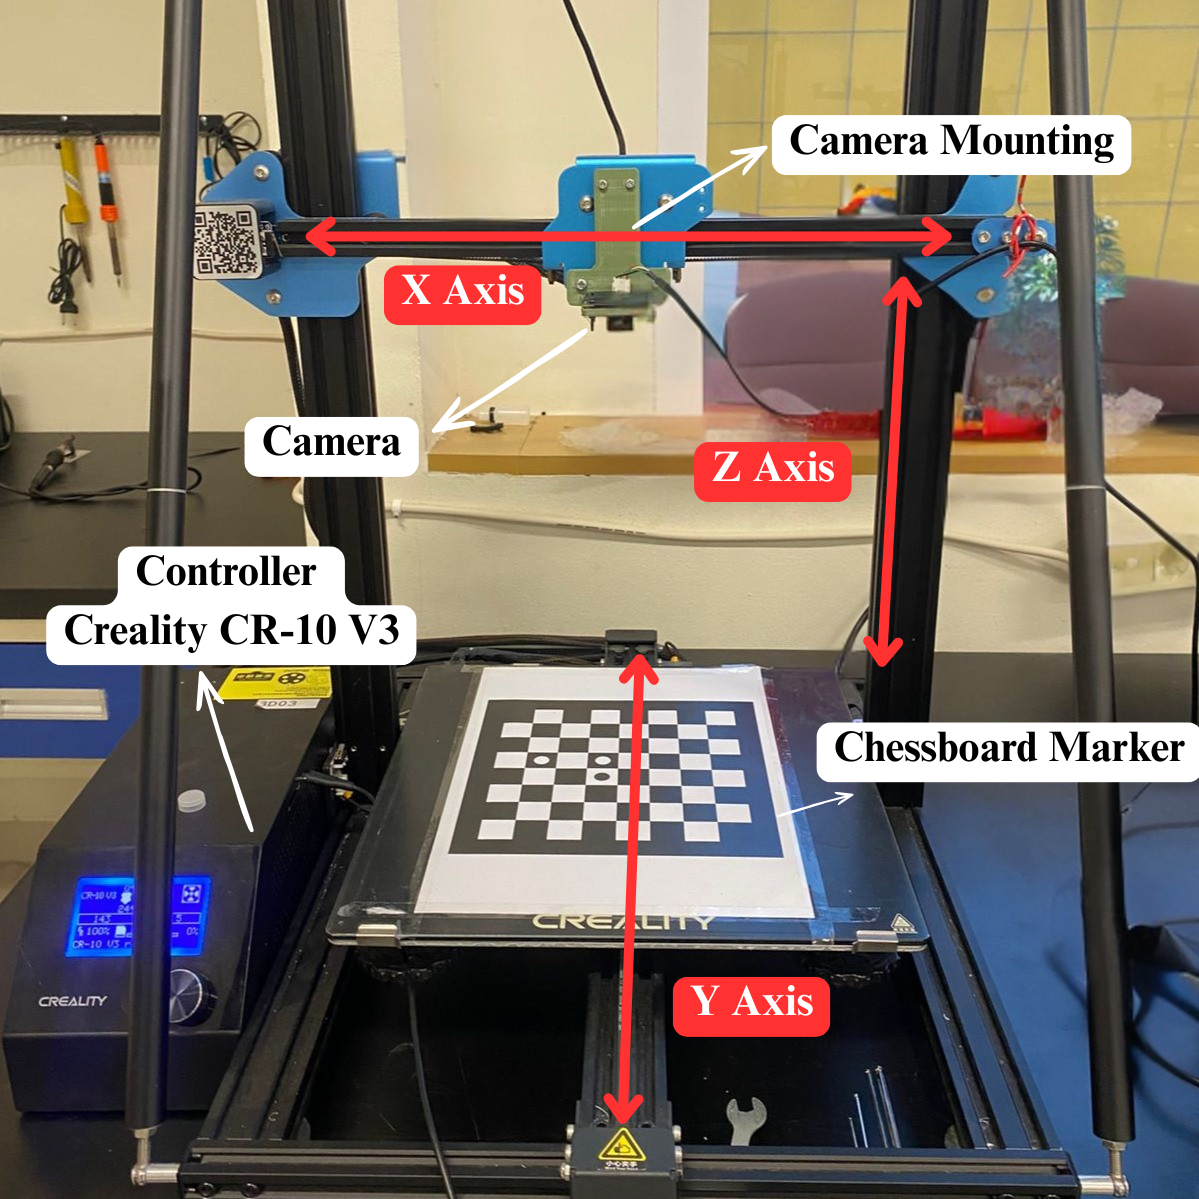
\includegraphics[width=0.75\linewidth]{images/setup.png}
    \caption{System Setup Configuration}
    \label{fig:setup}
\end{figure}

The specifications of the displayed chessboard marker are detailed as follows: 
\begin{enumerate}
    \item Calibration Board: A single calibration target featuring an $8 \times 8$ chessboard grid with a square size of 20 mm.
    \item Sorting Anchors: Three circular marker anchors with a radius of 5 mm positioned at the center of the board.
    \item Reference Specifications: Adopted from the benchmark parameters defined in \cite{Dan2022}.
\end{enumerate}


\subsection{Camera Calibration}


Prior to deploying the camera-based virtual encoder system, camera calibration must be conducted to establish baseline geometric parameters. The calibration workflow is partitioned into three main stages: Feature Extraction utilizing the EDLines algorithm, Homography Alignment to resolve chessboard orientation, and Calibration Evaluation to extract the camera intrinsic matrix, distortion coefficients, and overall reprojection error. The complete camera calibration procedure is summarized in Algorithm \ref{alg:calibration_pipeline}.

%%%%%%%% ini dihapus
\begin{algorithm}[t]
\caption{Camera Calibration Pipeline}
\label{alg:calibration_pipeline}
\begin{algorithmic}[1]
\footnotesize

\Function{FeatureExtraction}{$I_{\text{gray}}$}
    \State $L_{\text{raw}} \gets \text{EDLines}(I_{\text{gray}})$
    \State $C_{\text{init}}, L_{\text{valid}} \gets \text{ScreenLinesAndIntersect}(I_{\text{gray}}, L_{\text{raw}})$
    \State $C_{\text{sub}} \gets \text{SubpixelOptimization}(I_{\text{gray}}, C_{\text{init}})$
    \State \Return $C_{\text{sub}}$
\EndFunction

\Statex

\Function{HomographyAlignment}{$C_{\text{sub}}, I_{\text{gray}}, (M, N)$}
    \State $I_{\text{enh}} \gets \text{GaussianBlur}(\text{CLAHE}(I_{\text{gray}}), (5,5))$
    \State $E \gets \text{DetectEllipsesOrCircles}(I_{\text{enh}})$
    \State $C_{\text{grid}} \gets \text{FilterCentralPoints}(C_{\text{sub}}, E, M \times N)$
    \State $idx_{TL} \gets \arg\min(x+y)$
    \State $idx_{BR} \gets \arg\max(x+y)$
    \State $idx_{TR} \gets \arg\max(x-y)$
    \State $idx_{BL} \gets \arg\min(x-y)$
    \State $P_{\text{src}} \gets [C_{\text{grid}}[idx_{TL}], C_{\text{grid}}[idx_{TR}],$
    \Statex \hspace{3.5em} $C_{\text{grid}}[idx_{BR}], C_{\text{grid}}[idx_{BL}]]$
    \State $P_{\text{dst}} \gets [(0,0), (M-1,0), (M-1,N-1), (0,N-1)]$
    \State $H \gets \text{FindHomography}(P_{\text{dst}}, P_{\text{src}})$
    \State $C_{\text{sorted}} \gets \text{SnapGridToPoints}(C_{\text{grid}}, H, M, N)$
    \State \Return $C_{\text{sorted}}$
\EndFunction

\Statex

\Function{CalibrationEvaluation}{$\{\mathcal{P}_{3D}\}, \{\mathcal{C}_{2D}\}, \text{shape}$}
    \State $K, D, \{R_i\}, \{t_i\} \gets \text{CalibrateCamera}($
    \Statex \hspace{4em} $\{\mathcal{P}_{3D}\}, \{\mathcal{C}_{2D}\}, \text{shape})$
    \State $\text{SSE}_{\text{total}} \gets 0, \quad N_{\text{total}} \gets 0$
    \For{$i = 1 \dots |\mathcal{C}_{2D}|$}
        \State $\hat{p}_i \gets \text{ProjectPoints}(\mathcal{P}_{3D}[i], R_i, t_i, K, D)$
        \State $\text{SSE}_i \gets \|\mathcal{C}_{2D}[i] - \hat{p}_i\|_2^2$
        \State $\text{SSE}_{\text{total}} \gets \text{SSE}_{\text{total}} + \text{SSE}_i$
        \State $N_{\text{total}} \gets N_{\text{total}} + N_{\text{pts}}$
    \EndFor
    \State $\text{RMSE}_{\text{overall}} \gets \sqrt{\text{SSE}_{\text{total}} / N_{\text{total}}}$
    \State \Return $K, D, \text{RMSE}_{\text{overall}}$
\EndFunction

\Statex
\textbf{Main Execution Routine:}
\State Initialize $\mathcal{C}_{2D} \gets \emptyset$, $\mathcal{P}_{3D} \gets \emptyset$
\For{each image $I \in \text{Dataset}$}
    \State $I_{\text{gray}} \gets \text{ConvertToGray}(I)$
    \State $C_{\text{sub}} \gets \text{FeatureExtraction}(I_{\text{gray}})$
    \State $C_{\text{sorted}} \gets \text{HomographyAlignment}($
    \Statex \hspace{5.5em} $C_{\text{sub}}, I_{\text{gray}}, (M, N))$
    \If{$C_{\text{sorted}} \neq \text{None}$}
        \State Append $\mathcal{P}_{3D}$ and $C_{\text{sorted}}$ to $\{\mathcal{P}_{3D}\}$ and $\{\mathcal{C}_{2D}\}$
    \EndIf
\EndFor
\State $K, D, \text{RMSE}_{\text{overall}} \gets \text{CalibrationEvaluation}($
\Statex \hspace{4em} $\{\mathcal{P}_{3D}\}, \{\mathcal{C}_{2D}\}, \text{shape})$

\end{algorithmic}
\end{algorithm}

%%%%%%% dijadikan paragraf


\subsection{Virtual Encoder Workflow}
As outlined in Section \ref{proposed_encoder}, the virtual encoder leverages EDLines-based feature extraction—identical to the camera calibration pipeline—to extract precise chessboard corner coordinates. These refined corner points are subsequently utilized for 6-DOF pose estimation to track the relative spatial displacement of the chessboard marker across sequential image frames with respect to the camera frame. Pose estimation is resolved using an iterative Perspective-n-Point (SolvePnP) solver. The complete virtual encoder procedure is detailed in Algorithm \ref{alg:pose_extraction}.

\begin{algorithm}[t]
\caption{Virtual Encoder Workflow}
\label{alg:pose_extraction}
\begin{algorithmic}[1]
\footnotesize

\Require Image $I$, Intrinsic $\mathbf{K}$, Distortion $\mathbf{D}$, 3D points $\mathbf{P}_{3\text{D}}$,
\Statex \hspace{2.5em} Grid $(W, H) = (7, 7)$, Threshold $\epsilon_{\text{rmse}}$
\Ensure Position $p = (p_{\text{active}}, p_{\text{passive}})$, Error $\epsilon$

\Function{ExtractPosition}{$I, \mathbf{K}, \mathbf{D}, \mathbf{P}_{3\text{D}}$}
    \If{$I$ is invalid or empty} 
        \State \Return $\text{Null}, \infty$ 
    \EndIf

    \State $I_{\text{gray}} \gets \text{ConvertToGrayscale}(I)$
    \State $C_{\text{sub}} \gets \text{FeatureExtraction}(I_{\text{gray}})$
    \State $C_{\text{sorted}} \gets \text{HomographyAlignment}($
    \Statex \hspace{5.5em} $C_{\text{sub}}, I_{\text{gray}}, (W, H))$

    \If{$C_{\text{sorted}} = \text{Null}$}
        \State \Return $\text{Null}, \infty$
    \EndIf

    \State $\text{success}, \mathbf{rvec}, \mathbf{tvec} \gets \text{SolvePnP}(\mathbf{P}_{3\text{D}}, C_{\text{sorted}}, \mathbf{K}, \mathbf{D})$

    \If{$\text{success}$}
        \State $\mathbf{P}_{\text{proj}} \gets \text{ProjectPoints}(\mathbf{P}_{3\text{D}}, \mathbf{rvec}, \mathbf{tvec}, \mathbf{K}, \mathbf{D})$
        \State $\epsilon \gets \sqrt{\frac{1}{M} \|C_{\text{sorted}} - \mathbf{P}_{\text{proj}}\|_2^2}$

        \If{$\epsilon \le \epsilon_{\text{rmse}}$}
            \State Extract 2D translation $p \gets (\mathbf{tvec}[0], \mathbf{tvec}[1])$
            \State \Return $p, \epsilon$
        \EndIf
    \EndIf

    \State \Return $\text{Null}, \infty$
\EndFunction

\end{algorithmic}
\end{algorithm}

\subsection{Virtual Encoder Measurement Error Testing and Metrological Framework}
In this stage, the measurement accuracy of the virtual encoder system is evaluated by comparing its displacement readouts against reference measurements obtained using a high-precision mechanical dial gauge. The physical machine movement sequence employed for this evaluation is described in Algorithm \ref{alg:sequence}.

\begin{algorithm}[t]
	\caption{Data Capturing Sequence for Kinematic Error Extraction}
	\label{alg:sequence}
	\begin{algorithmic}[1]
		\footnotesize
		
		\Require Commanded displacement $D_{\text{cmd}}$, total iterations $N$
		\Ensure Captured frames $\mathcal{F} = \{F_{\text{init}, i}, F_{\text{fwd}, i}, F_{\text{rev}, i}\}$ and
		\Statex \hspace{2.5em} positions $\{p_{\text{init}, i}, p_{\text{fwd}, i}, p_{\text{rev}, i}\}$
		
		\State Move machine active axis to reference anchor position $p_0$
		\State Capture Initial Frame $F_{\text{init}, 1} \implies p_{\text{init}, 1}$
		
		\For{$i = 1$ \textbf{to} $N$}
		\State Move Forward by $+D_{\text{cmd}}$
		\State Capture Forward Frame $F_{\text{fwd}, i} \implies p_{\text{fwd}, i}$
		\State Move Backward by $-D_{\text{cmd}}$
		\State Capture Reversal Frame $F_{\text{rev}, i} \implies p_{\text{rev}, i}$
		\If{$i < N$}
		\State Perform Preload Out (Move $-D_{\text{cmd}}$)
		\State Perform Preload In (Move $+D_{\text{cmd}}$)
		\State Capture Initial Frame $F_{\text{init}, i+1} \implies p_{\text{init}, i+1}$
		\EndIf
		\EndFor
		
	\end{algorithmic}
\end{algorithm}

For this evaluation sequence, a commanded displacement ($D_{\text{cmd}}$) of 0.5~mm is selected, conforming to the physical travel limits of the dial gauge, which features a maximum single-revolution range of 0.8~mm. Positional readouts extracted from the forward and reversal frames are subsequently compared, and their mean deviation is calculated to determine the absolute measurement error of the virtual encoder.

To establish a rigorous metrological foundation, a measurement uncertainty framework is formulated in accordance with the ISO/IEC Guide 98-3 (GUM) standard. The combined standard uncertainty ($u_c$) incorporates both Type A evaluations (derived from statistical experimental repeatability) and Type B evaluations (derived from systemic physical, optical, and hardware boundaries). The combined uncertainty model is expressed analytically as:
\begin{equation}
	u_c = \sqrt{u_A^2 + u_{\text{noise}}^2 + u_{\text{reproj}}^2 + u_{\text{dial}}^2}
	\label{eq:gum_uc}
\end{equation}
where:
\begin{itemize}
	\item $u_A = \frac{\sigma}{\sqrt{N}}$ defines the Type A standard uncertainty from $N$ repeated displacement measurements.
	\item $u_{\text{noise}}$ denotes the Type B standard uncertainty induced by static optical fluctuations and mechanical micro-vibrations.
	\item $u_{\text{reproj}}$ quantifies the sub-pixel reprojection residual uncertainty, modeled across the spatial averaging of the $7 \times 7$ chessboard corner grid.
	\item $u_{\text{dial}} = \frac{a}{\sqrt{3}}$ represents the Type B uncertainty from the reference dial gauge tolerance ($a = 10~\mu\text{m}$), assuming a uniform rectangular distribution.
\end{itemize}

The expanded uncertainty ($U$) at a 95\% confidence level is subsequently evaluated using a coverage factor of $k = 2$:
\begin{equation}
	U = k \cdot u_c = 2 \cdot u_c
	\label{eq:gum_expanded}
\end{equation}

\subsection{Machine Calibration Protocol}
The proposed calibration framework comprises three distinct evaluation phases: Measurement Error, Linear Axis Error, and Circular Trajectory Error profiling. Both linear axis and circular trajectory performance are evaluated under baseline (uncalibrated) conditions and post-calibration states to verify compensation effectiveness. The overall calibration protocol workflow is illustrated in \figref{fig:protocol}.

\begin{figure}[ht]
    \centering
    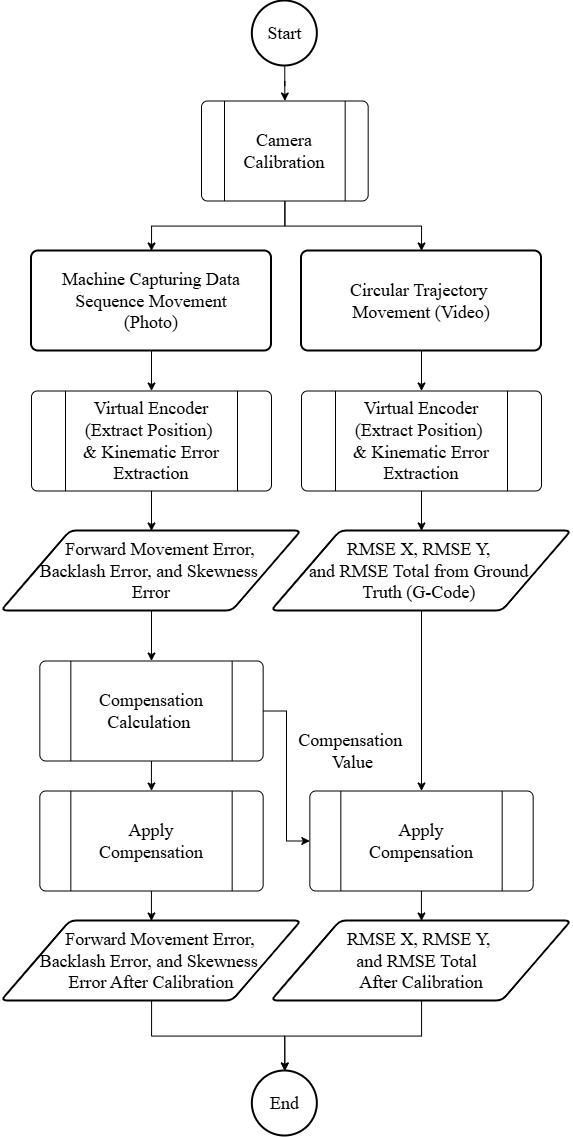
\includegraphics[width=0.75\linewidth]{images/Calibration Protocol Fix.drawio.png}
    \caption{Calibration Protocol Diagram}
    \label{fig:protocol}
\end{figure}

\begin{algorithm}[t]
	\caption{Kinematic Parameter Extraction and Compensation}
	\label{alg:kompensasi}
	\begin{algorithmic}[1]
		\footnotesize
		
		\Function{KinematicErrorExtraction}{$\mathcal{S}, \mathbf{K}, \mathbf{D}, \mathbf{P}_{3\text{D}}, \epsilon_{\text{thresh}}, N_{\text{max}}$}
		\State Initialize $\mathcal{D}_{\text{act}} \gets \emptyset$, $\mathcal{B} \gets \emptyset$, $\mathcal{S}_{\text{skew}} \gets \emptyset$, $N_{\text{valid}} \gets 0$
		
		\For{each triplet $(F_{\text{init}}, F_{\text{fwd}}, F_{\text{rev}}) \in \mathcal{S}$}
		\State $p_{\text{init}}, \epsilon_{\text{init}} \gets \text{ExtractPosition}(F_{\text{init}}, \mathbf{K}, \mathbf{D}, \mathbf{P}_{3\text{D}})$
		\State $p_{\text{fwd}}, \epsilon_{\text{fwd}} \gets \text{ExtractPosition}(F_{\text{fwd}}, \mathbf{K}, \mathbf{D}, \mathbf{P}_{3\text{D}})$
		\State $p_{\text{rev}}, \epsilon_{\text{rev}} \gets \text{ExtractPosition}(F_{\text{rev}}, \mathbf{K}, \mathbf{D}, \mathbf{P}_{3\text{D}})$
		
		\State $\epsilon_{\text{max}} \gets \max(\epsilon_{\text{init}}, \epsilon_{\text{fwd}}, \epsilon_{\text{rev}})$
		\If{$p_{\text{init}} \neq \text{Null} \land p_{\text{fwd}} \neq \text{Null} \land p_{\text{rev}} \neq \text{Null} \land \epsilon_{\text{max}} \le \epsilon_{\text{thresh}}$}
		\State $\Delta p_{\text{act}} \gets p_{\text{fwd,act}} - p_{\text{init,act}}$
		\State $\Delta p_{\text{pas}} \gets p_{\text{fwd,pas}} - p_{\text{init,pas}}$
		\State $B_i \gets |p_{\text{rev,act}} - p_{\text{init,act}}|$
		\State $S_i \gets \Delta p_{\text{pas}} / \Delta p_{\text{act}}$
		
		\State Append $\Delta p_{\text{act}}$ to $\mathcal{D}_{\text{act}}$, $B_i$ to $\mathcal{B}$, $S_i$ to $\mathcal{S}_{\text{skew}}$
		\State $N_{\text{valid}} \gets N_{\text{valid}} + 1$
		
		\If{$N_{\text{valid}} \ge N_{\text{max}}$}
		\State \textbf{break}
		\EndIf
		\EndIf
		\EndFor
		\State \Return $\mathcal{D}_{\text{act}}, \mathcal{B}, \mathcal{S}_{\text{skew}}$
		\EndFunction
		
		\Statex
		
		\Function{CompensationCalculation}{$\mathcal{D}_{\text{act}}, \mathcal{B}, \mathcal{S}_{\text{skew}}, D_{\text{cmd}}, S_{\text{curr}}$}
		\If{$\mathcal{D}_{\text{act}} = \emptyset$}
		\State \Return $\text{Null}, \text{Null}, \text{Null}$
		\EndIf
		
		\State $\bar{\Delta p}_{\text{act}} \gets \text{Mean}(\mathcal{D}_{\text{act}})$
		\State $\bar{B} \gets \text{Mean}(\mathcal{B})$
		\State $\bar{S} \gets \text{Mean}(\mathcal{S}_{\text{skew}})$
		
		\State $S_{\text{new}} \gets (D_{\text{cmd}} / \bar{\Delta p}_{\text{act}}) \cdot S_{\text{curr}}$
		\State $B_{\text{comp}} \gets \bar{B}$
		\State $I_{\text{skew}} \gets \bar{S}$
		
		\State \Return $S_{\text{new}}, B_{\text{comp}}, I_{\text{skew}}$
		\EndFunction
		
		\Statex
		
		\Function{ApplyCompensation}{$\mathbf{p}, A, \mathbf{\Theta}, b$}
		\State Extract $(\Delta x, \Delta y) \gets \mathbf{p}$ and $(S_{\text{new}}, B_{\text{comp}}, I_{\text{skew}}) \gets \mathbf{\Theta}$
		\If{$S_{\text{new}} \neq \text{Null}$}
		\State Send G-code: \texttt{M92} $A = S_{\text{new}}$
		\EndIf
		
		\State $\Delta x_{\text{comp}} \gets \Delta x, \quad \Delta y_{\text{comp}} \gets \Delta y$
		
		\If{$A = X$}
		\State $\Delta y_{\text{comp}} \gets \Delta y_{\text{comp}} - (\Delta x \cdot I_{\text{skew}})$
		\ElsIf{$A = Y$}
		\State $\Delta x_{\text{comp}} \gets \Delta x_{\text{comp}} - (\Delta y \cdot I_{\text{skew}})$
		\EndIf
		
		\If{$b = \text{True}$}
		\If{$A = X$}
		\If{$\Delta x_{\text{comp}} < 0$}
		\State $\Delta x_{\text{comp}} \gets \Delta x_{\text{comp}} - B_{\text{comp}}$
		\Else
		\State $\Delta x_{\text{comp}} \gets \Delta x_{\text{comp}} + B_{\text{comp}}$
		\EndIf
		\ElsIf{$A = Y$}
		\If{$\Delta y_{\text{comp}} < 0$}
		\State $\Delta y_{\text{comp}} \gets \Delta y_{\text{comp}} - B_{\text{comp}}$
		\Else
		\State $\Delta y_{\text{comp}} \gets \Delta y_{\text{comp}} + B_{\text{comp}}$
		\EndIf
		\EndIf
		\EndIf
		
		\State \Return $\Delta x_{\text{comp}}, \Delta y_{\text{comp}}$
		\EndFunction
		
	\end{algorithmic}
\end{algorithm}

\subsection{Machine Linear Movement Performance Examination}
To extract linear step drift, mechanical backlash, and structural axis skewness error, this research utilizes a structured machine movement sequence to capture three distinct types of optical image frames, as detailed before in Algorithm~\ref{alg:sequence}:
\begin{enumerate}
    \item Initial Frame ($F_{\text{init}}$): Captured at the starting reference anchor coordinate, yielding the baseline spatial position $p_{\text{init}}$.
    \item Forward Frame ($F_{\text{fwd}}$): Captured after executing a forward displacement along the active axis, yielding the forward coordinate $p_{\text{fwd}}$.
    \item Reversal Frame ($F_{\text{rev}}$): Captured after returning to the nominal initial position, yielding the post-reversal coordinate $p_{\text{rev}}$.
\end{enumerate}
The measured spatial positions ($p_{\text{init}}$, $p_{\text{fwd}}$, and $p_{\text{rev}}$) extracted from these captured frames are subsequently used to compute the steps per millimeter correction, mechanical backlash, and axis skew factor. 

Prior to parameter aggregation, each image triplet undergoes strict outlier filtering based on the reprojection error threshold $\epsilon_{\text{rmse}}$. Valid position measurements are subsequently processed to isolate individual error metrics across $N_{\text{valid}}$ valid iterations. The analytical formulation for updating the steps-per-millimeter resolution, mechanical backlash compensation, and axis skew factor is formalized in Algorithm \ref{alg:kompensasi}. To obtain optimal parameters during the calibration process, fine-tuning is performed by repeating the same process until the machine reaches a steady state.

\subsection{Machine Circular Movement Performance Examination}
Because real-world additive manufacturing operations require coordinated multi-axis motion rather than single-axis displacements, evaluating tracking performance along continuous paths is essential for comprehensive machine profiling. To assess dynamic synchronization, a complex elliptical trajectory is executed, as depicted in \figref{fig:circexam}. The machine traces the commanded path via G-code execution while the virtual encoder records positional states at each video frame. The tracked trajectory is subsequently benchmarked against the ground-truth path using Root Mean Square Error (RMSE) analysis. The algorithmic workflow for this tracking evaluation is detailed in Algorithm \ref{alg:circular_eval}.

\begin{figure}[ht]
    \centering
    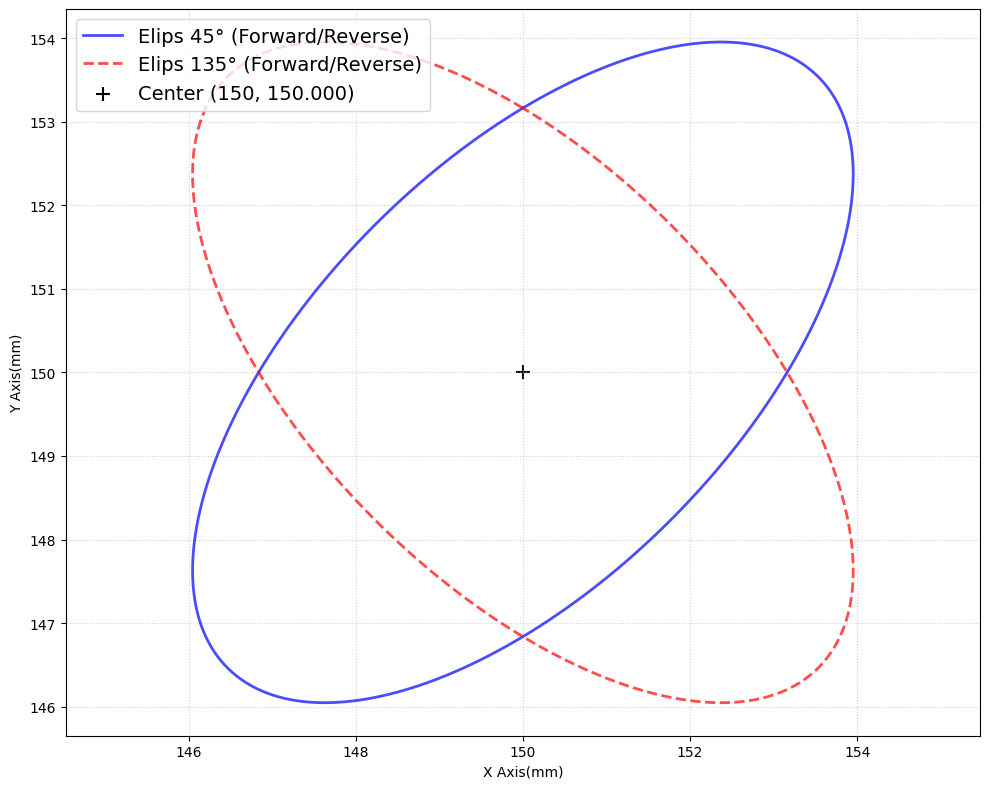
\includegraphics[width=0.8\linewidth]{images/circularmovement.png}
    \caption{Circular Examination Ellipse Model}
    \label{fig:circexam}
\end{figure}

\begin{algorithm}[t]
\caption{Circular Trajectory Extraction and Evaluation}
\label{alg:circular_eval}
\begin{algorithmic}[1]
\footnotesize

\Function{TrajectoryEvaluation}{$\mathcal{V}_{\text{dataset}}, \mathbf{P}_{\text{gt}}, \mathbf{K}, \mathbf{D}, \mathbf{P}_{3\text{D}}, \epsilon_{\text{thresh}}$}
    \State $T_{\text{gt}} \gets \text{BuildKDTree}(\mathbf{P}_{\text{gt}})$ \Comment{Build spatial tree index}
    \State Initialize $\mathcal{E}_x \gets \emptyset, \mathcal{E}_y \gets \emptyset, \mathcal{E}_{\text{tot}} \gets \emptyset$

    \For{each video $V \in \mathcal{V}_{\text{dataset}}$}
        \State Initialize $\mathbf{P}_{\text{enc}} \gets \emptyset$, $p_0 \gets \text{Null}$

        \State \Comment{1. Frame-by-Frame Virtual Encoder Trajectory Extraction}
        \For{each frame $I_k \in V$}
            \State $p_k, \epsilon_k \gets \text{ExtractPosition}(I_k, \mathbf{K}, \mathbf{D}, \mathbf{P}_{3\text{D}})$

            \If{$p_k \neq \text{Null} \land \epsilon_k \le \epsilon_{\text{thresh}}$}
                \If{$p_0 = \text{Null}$}
                    \State $p_0 \gets p_k$ \Comment{Set baseline origin}
                \EndIf
                \State $\mathbf{p}_{\text{rel}} \gets p_k - p_0$ \Comment{Compute relative displacement}
                \State Append $\mathbf{p}_{\text{rel}} \to \mathbf{P}_{\text{enc}}$
            \EndIf
        \EndFor

        \State Export $\mathbf{P}_{\text{enc}}$ to CSV \Comment{Save extracted trajectory}

        \State \Comment{2. Trajectory Tracking Evaluation}
        \State $\mathbf{P}_{\text{enc}} \gets \mathbf{P}_{\text{enc}} - \mathbf{P}_{\text{enc}}[0] + \mathbf{P}_{\text{gt}}[0]$ \Comment{Align initial origin}
        \State $\mathbf{P}_{\text{cls}}, \mathbf{d} \gets \text{QueryNearest}(T_{\text{gt}}, \mathbf{P}_{\text{enc}})$ \Comment{Nearest-neighbor search}

        \State $e_x \gets \sqrt{\text{Mean}((\mathbf{P}_{\text{enc}, x} - \mathbf{P}_{\text{cls}, x})^2)} \times 1000$
        \State $e_y \gets \sqrt{\text{Mean}((\mathbf{P}_{\text{enc}, y} - \mathbf{P}_{\text{cls}, y})^2)} \times 1000$
        \State $e_{\text{tot}} \gets \sqrt{\text{Mean}(\mathbf{d}^2)} \times 1000$

        \State Append $e_x \to \mathcal{E}_x, \quad e_y \to \mathcal{E}_y, \quad e_{\text{tot}} \to \mathcal{E}_{\text{tot}}$
    \EndFor

    \State $\bar{E}_x \gets \text{Mean}(\mathcal{E}_x), \quad \bar{E}_y \gets \text{Mean}(\mathcal{E}_y), \quad \bar{E}_{\text{tot}} \gets \text{Mean}(\mathcal{E}_{\text{tot}})$
    \State \Return $\bar{E}_x, \bar{E}_y, \bar{E}_{\text{tot}}$ \Comment{RMSE in $\mu\text{m}$}
\EndFunction

\end{algorithmic}
\end{algorithm}
\section{Experimental Results and Discussion}
\label{results}

\subsection{Camera Calibration Performance}
To establish the baseline internal camera model, a robust 10-frame image dataset was processed for geometric calibration. Frames exhibiting severe optical distortion or fewer than 49 detectable corners were discarded during outlier screening. The calibration pipeline achieved a mean reprojection error of 0.1152~pixels ($\sigma = 0.0076$~pixels), confirming high geometric modeling accuracy. A representative calibration visualization following feature extraction and homography alignment is illustrated in \figref{fig:Calib}.

\begin{figure}[ht]
	\centering
	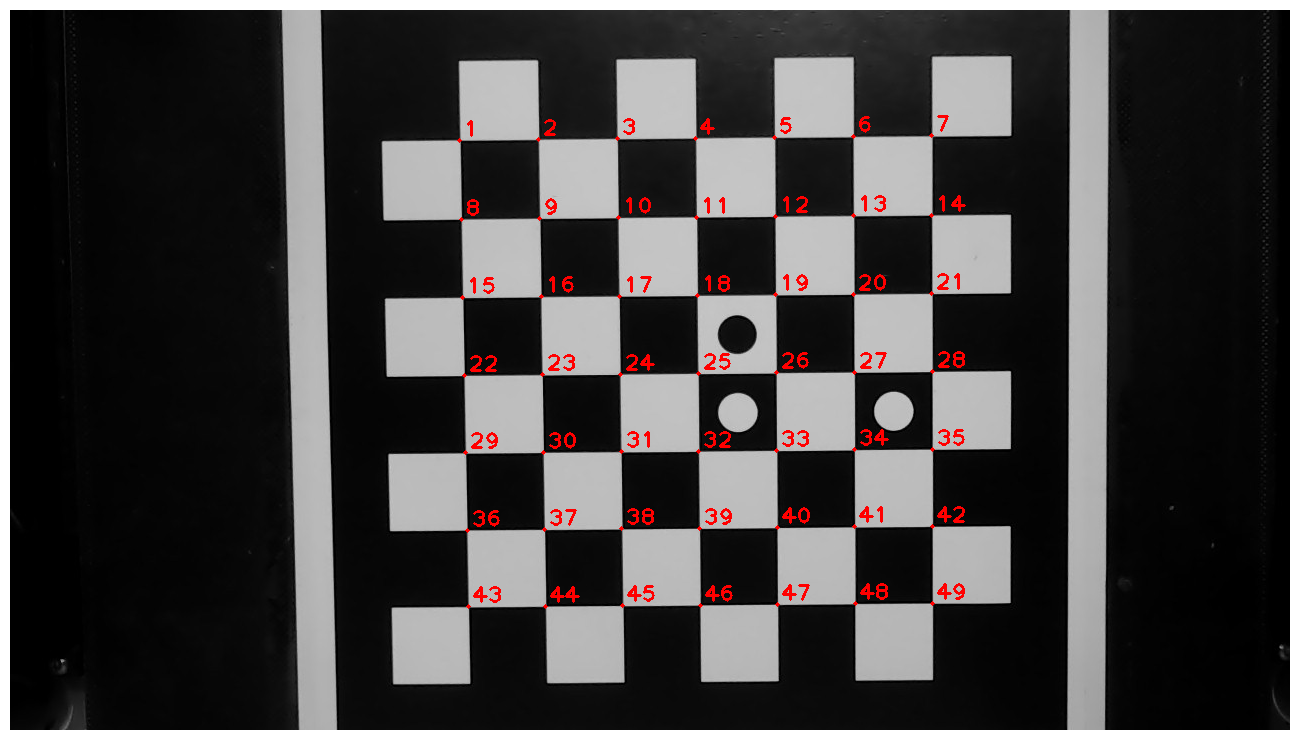
\includegraphics[width=0.8\linewidth]{images/result_after_corner_sorting.png}
	\caption{Calibration visualization following feature extraction and homography alignment.}
	\label{fig:Calib}
\end{figure}

The estimated internal camera parameters, comprising the intrinsic camera matrix $K$ and the lens distortion vector $D$, were resolved as \eqref{eq:intrinsic_matrix} and \eqref{eq:distortion_coeffs}:

\begin{equation}
	\label{eq:intrinsic_matrix}
	K = \begin{bmatrix} 2314.64 & 0 & 637.08 \\ 0 & 2328.29 & 222.87 \\ 0 & 0 & 1 \end{bmatrix}
\end{equation}

\begin{equation}
	\label{eq:distortion_coeffs}
	D = \begin{bmatrix} -0.0561 & 0.9595 & 0.0001 & 0.0004 \end{bmatrix}
\end{equation}

As derived in \eqref{eq:intrinsic_matrix}, the close match between the directional focal lengths ($f_x = 2314.64$ and $f_y = 2328.29$) confirms a uniform 1:1 sensor aspect ratio. Furthermore, the coefficients in \eqref{eq:distortion_coeffs} reveal a distinct mustache distortion profile resulting from the alternating signs between the radial distortion parameters $k_1$ and $k_2$.

\subsection{Measurement Error and Noise Floor Analysis}
The experimental displacement tracking performance was evaluated against physical dial gauge measurements over a 0.5~mm travel range. The visual output display from the position extraction pipeline of the virtual encoder is illustrated in \figref{fig:positionextraction}. The statistical measurement comparison across all evaluation cycles is presented in \figref{fig:position_comparison}. Empirical validation confirms an absolute measurement error of $3.55~\mu\text{m}$ for the X-axis and $6.25~\mu\text{m}$ for the Y-axis.

\begin{figure}[ht]
	\centering
	\subfloat[]{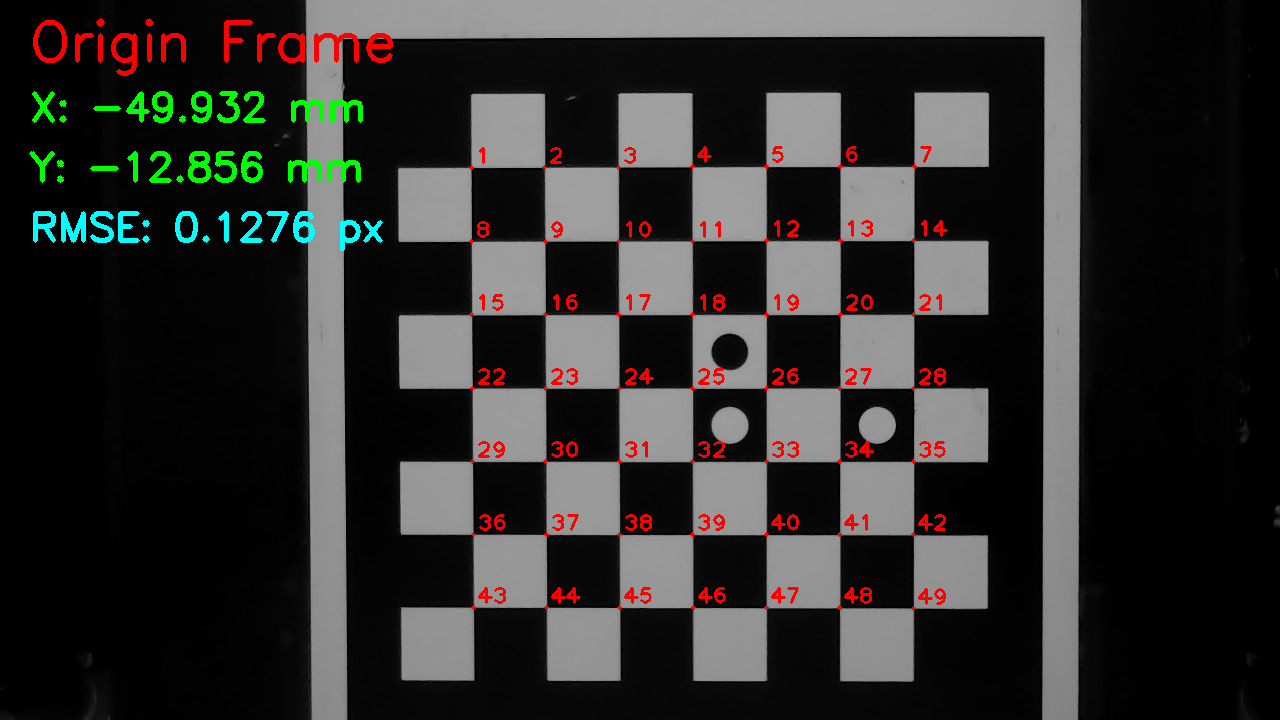
\includegraphics[width=0.75\linewidth]{images/visualisasi_ori.png}\label{fig:vis_ori}}
	\\
	\subfloat[]{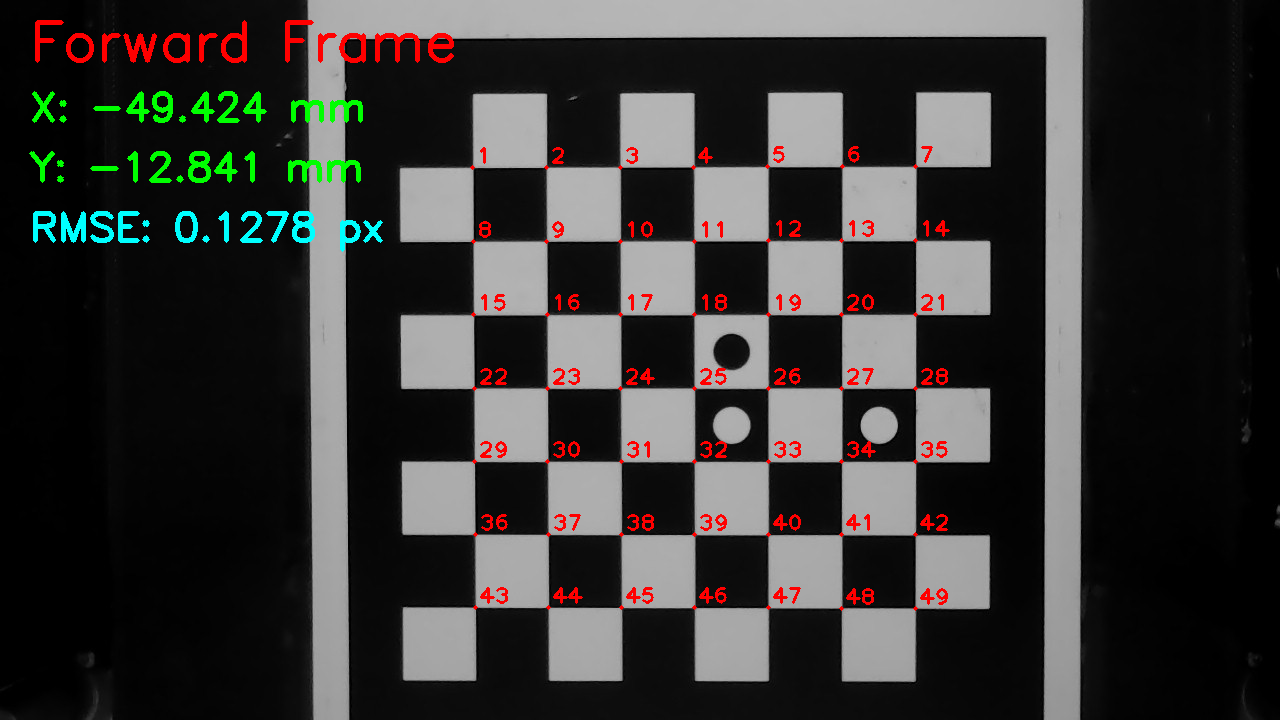
\includegraphics[width=0.75\linewidth]{images/visualisasi_fwd.png}\label{fig:vis_fwd}}
	\\
	\subfloat[]{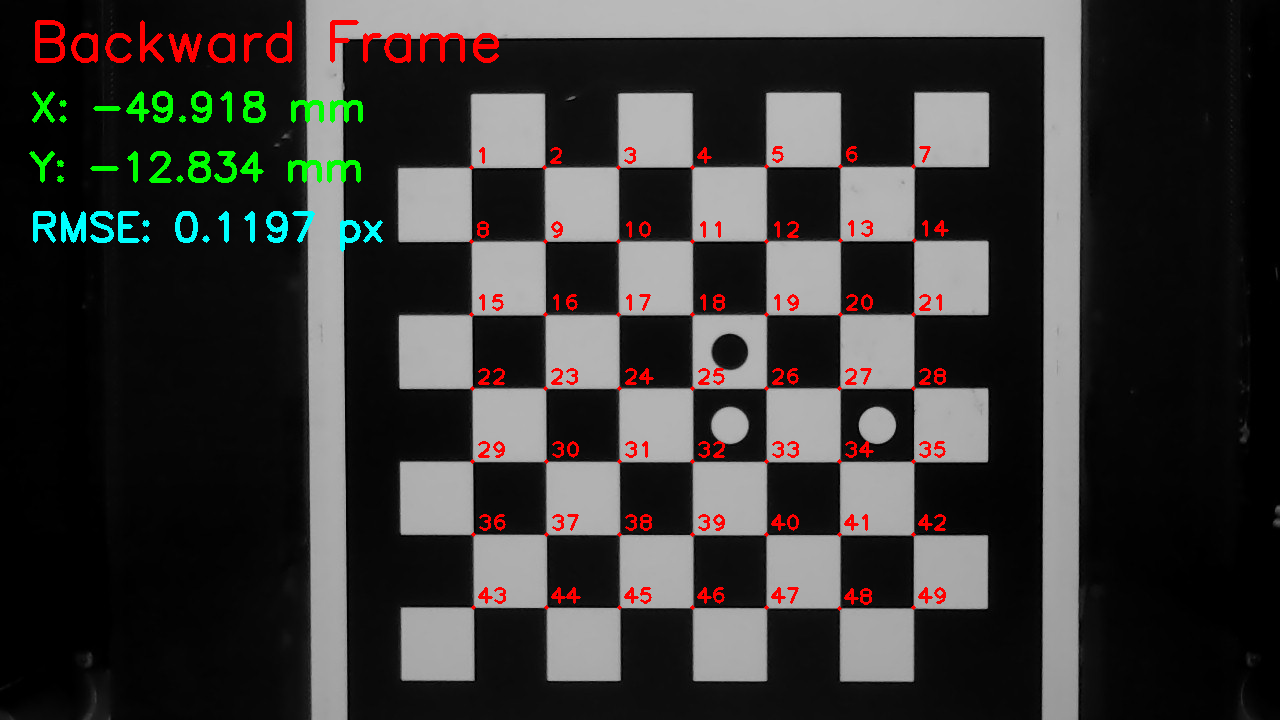
\includegraphics[width=0.75\linewidth]{images/visualisasi_bck.png}\label{fig:vis_bck}}
	\caption{Visualization of position extraction from virtual encoder process on one of the axes: (a) original frame position, (b) forward frame position, and (c) backward frame position.}
	\label{fig:positionextraction}
\end{figure}

\begin{figure}[t]
	\centering
	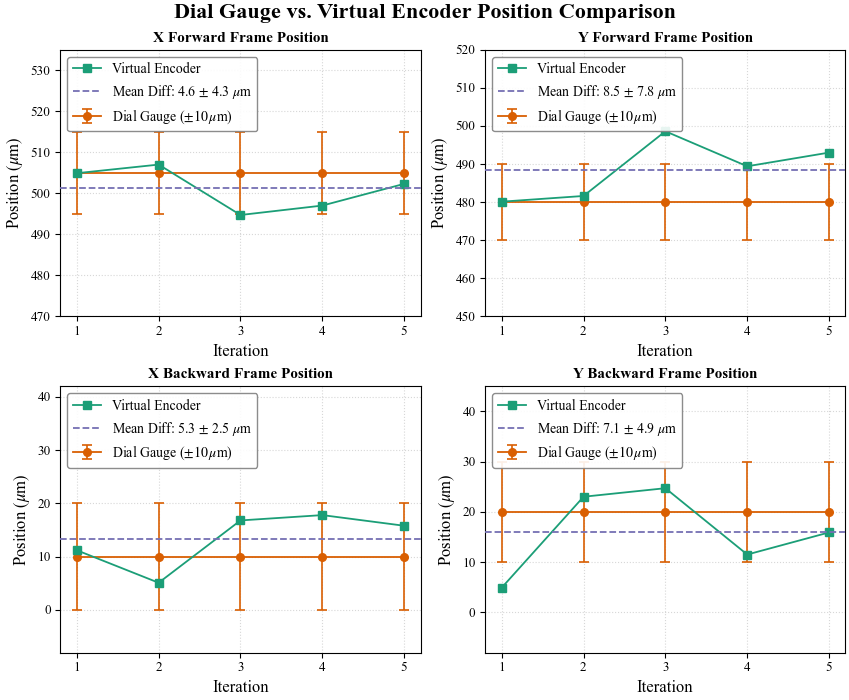
\includegraphics[width=1\linewidth]{images/1_4_position_comparison_combined.png}
	\caption{Comparison of position measurements between the dial gauge and virtual encoder across X and Y axes: forward frame position, Y forward frame position, X backward frame position, and Y backward frame position.}
	\label{fig:position_comparison}
\end{figure}

Static environmental testing under stationary conditions (\figref{fig:Noise}) yielded an internal static noise floor of $2.58~\mu\text{m}$ ($\sigma = 2.50~\mu\text{m}$) for the X-axis and $4.97~\mu\text{m}$ ($\sigma = 3.30~\mu\text{m}$) for the Y-axis. This physical deviation stems primarily from localized ambient illumination variations and structural micro-vibrations in the machine chassis. 

Based on the OV9821 sensor hardware specification with a physical pixel pitch $p_{\text{sensor}} = 3.0~\mu\text{m}$, the intrinsic focal length $f_x = 2314.64~\text{pixels}$ converts to an effective focal length $f \approx 6.94~\text{mm}$. At a fixed camera working distance $Z = 260~\text{mm}$, the physical projection scale on the print bed plane translates to $112.33~\mu\text{m/pixel}$. Consequently, the measured static noise floor corresponds to an equivalent sub-pixel detection sensitivity of $0.023~\text{pixels}$ (X-axis) and $0.044~\text{pixels}$ (Y-axis). On the physical CMOS sensor plane, a target displacement error of $2.58~\mu\text{m}$ projects to a sub-diffraction physical shift of merely $68.8~\text{nm}$ ($2.58~\mu\text{m} \times M$, where optical magnification $M = 0.0267$), demonstrating the sub-pixel precision of the EDLines corner detection pipeline. Across the $0.5~\text{mm}$ operational displacement range, the virtual encoder achieves a spatial signal-to-noise ratio ($\text{SNR}_{\text{spatial}}$) of $45.75~\text{dB}$ for the X-axis and $40.05~\text{dB}$ for the Y-axis.

\begin{figure}[tbp]
	\centering
	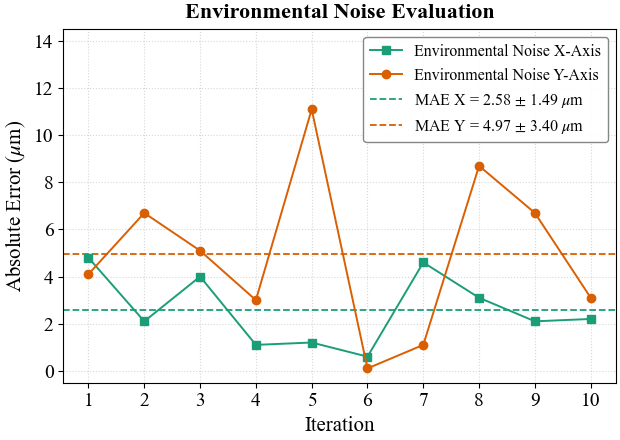
\includegraphics[width=0.8\linewidth]{images/Noise_Lingkungan.png}
	\caption{System noise floor characterization measured under stationary static testing for X and Y axes.}
	\label{fig:Noise}
\end{figure}

To comprehensively evaluate the metrological performance of the proposed virtual encoder system, both Type A and Type B measurement uncertainties were systematically quantified. The evaluation incorporates individual contributions arising from experimental repeatability, static optical noise, sub-pixel reprojection residuals, and reference hardware tolerances. The populated measurement uncertainty budget, structured according to the GUM formulation in \eqref{eq:gum_uc} and \eqref{eq:gum_expanded}, is summarized in \tabref{tab:uncertainty_budget}.

\begin{table}[tbp]
	\centering
	\caption{Measurement Uncertainty Budget for the Virtual Encoder System (ISO/IEC Guide 98-3 GUM)}
	\label{tab:uncertainty_budget}
	\scriptsize
	\setlength{\tabcolsep}{2.5pt}
	\renewcommand{\arraystretch}{1.2}
	
	\begin{tabularx}{\linewidth}{@{} L c c c c @{}}
		\toprule
		\textbf{Source of Uncertainty} & \textbf{Symbol} & \textbf{Distribution} & \textbf{X ($\mu$m)} & \textbf{Y ($\mu$m)} \\ 
		\midrule
		Measurement Repeatability (Type A) & $u_A$ & Normal ($N=5$) & 1.52 & 2.66 \\
		Static Optical Noise Floor & $u_{\text{noise}}$ & Normal & 1.49 & 3.40 \\
		Sub-pixel Reprojection Residual & $u_{\text{reproj}}$ & Normal & 2.96 & 2.96 \\
		Reference Dial Gauge Tolerance & $u_{\text{dial}}$ & Rectangular ($\sqrt{3}$) & 5.77 & 5.77 \\ 
		\midrule
		\textbf{Combined Std. Uncertainty ($u_c$)} & $u_c$ & Normal & \textbf{6.83} & \textbf{7.61} \\
		\textbf{Expanded Uncertainty ($U, k=2$)} & $U$ & Normal ($95\%$) & \textbf{13.66} & \textbf{15.22} \\ 
		\bottomrule
	\end{tabularx}
\end{table}

As indicated in \tabref{tab:uncertainty_budget}, the calculated expanded measurement uncertainty at a 95\% confidence level ($k=2$) is $13.66~\mu\text{m}$ along the X-axis and $15.22~\mu\text{m}$ along the Y-axis. Quantitative analysis of the budget components reveals that the physical reference instrument (dial gauge resolution tolerance) constitutes the primary Type B uncertainty contribution ($5.77~\mu\text{m}$). Conversely, the intrinsic optical uncertainty of the virtual encoder is maintained below $3.0~\mu\text{m}$, benefiting from the spatial corner-averaging effect inherent to the $7 \times 7$ chessboard marker array. Consequently, these findings confirm that the primary bottleneck in system accuracy arises from mechanical calibration limits rather than the vision-based tracking pipeline.

\subsection{Baseline Evaluation and Fine-Tuning Outcomes}
Initial testing of the uncalibrated machine revealed significant motion discrepancies. The default X-axis profile exhibited a forward travel error of $46.3~\mu$m and a backlash error of $12.4~\mu$m. The Y-axis displayed larger deviations, with a forward travel error of $55.0~\mu$m and a backlash gap of $24.4~\mu$m. Notably, structural axis skew introduced massive parasitic drifts under single-axis travel, showing an X-on-Y drift angle of $-0.5344^\circ$ and a Y-on-X drift angle of $0.5171^\circ$.

\begin{table}[b]
	\centering
	\caption[Fine-Tuned Calibration Parameters]{Fine-Tuned Calibration Parameters}
	\label{tab:parameter_final_kalibrasi}
	\footnotesize
	
	\begin{tabularx}{\linewidth}{@{} l X c @{}}
		\toprule
		\textbf{Parameter} & \textbf{Description} & \textbf{Final Value} \\
		\midrule
		\texttt{STEPX}        & X-axis step resolution & 79.72 \textit{steps/mm} \\
		\texttt{STEPY}        & Y-axis step resolution & 80.40 \textit{steps/mm} \\
		\midrule
		\texttt{BACKLASH\_X} & X-axis backlash compensation & 13.3 $\mu$m \\
		\texttt{BACKLASH\_Y} & Y-axis backlash compensation & 31.4 $\mu$m \\
		\midrule
		\texttt{SKEW\_X\_ON\_Y} & Parasitic X-drift during Y motion & -9.2 $\mu$m/mm \\
		\texttt{SKEW\_Y\_ON\_X} & Parasitic Y-drift during X motion & 9.213 $\mu$m/mm \\
		\bottomrule
	\end{tabularx}
\end{table}

\begin{figure}[t]
	\centering
	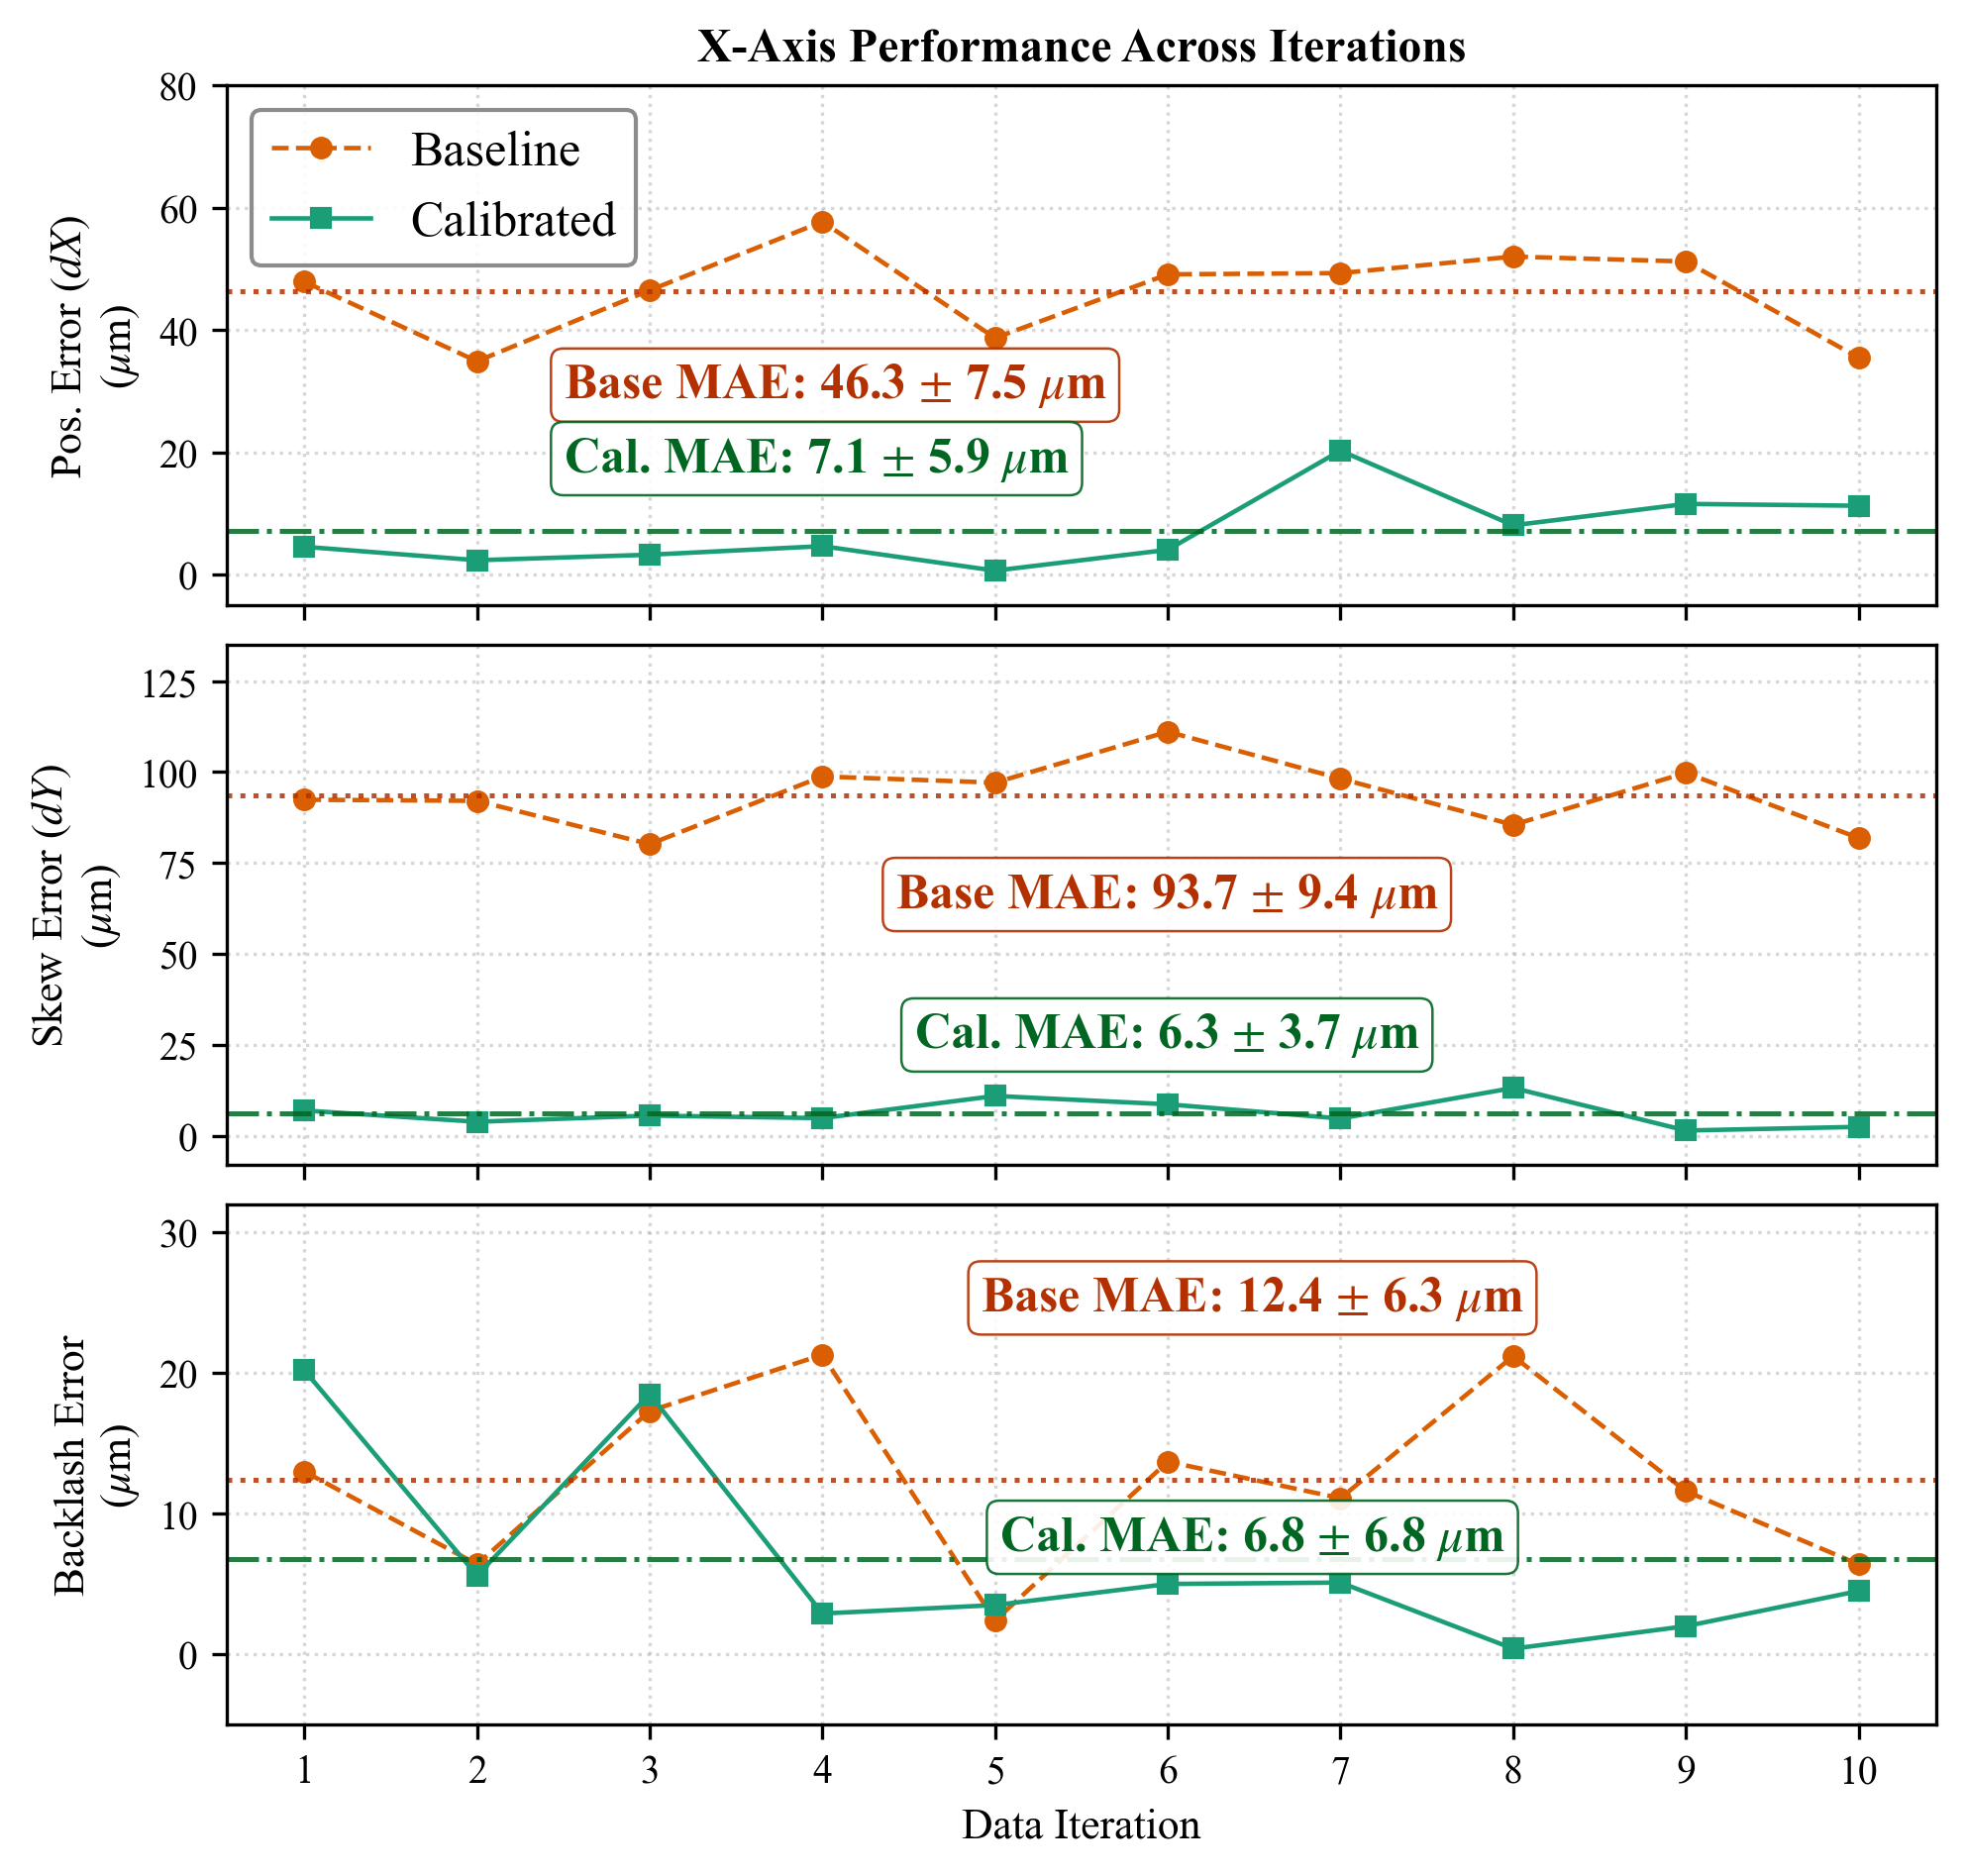
\includegraphics[width=1\linewidth]{images/x_axis_iterations.png}
	\caption{X-axis single-axis error tracking across 10 iterations comparing baseline and calibrated states for positioning, skew, and backlash parameters.}
	\label{fig:x_axis_iter}
\end{figure}

\begin{figure}[t]
	\centering
	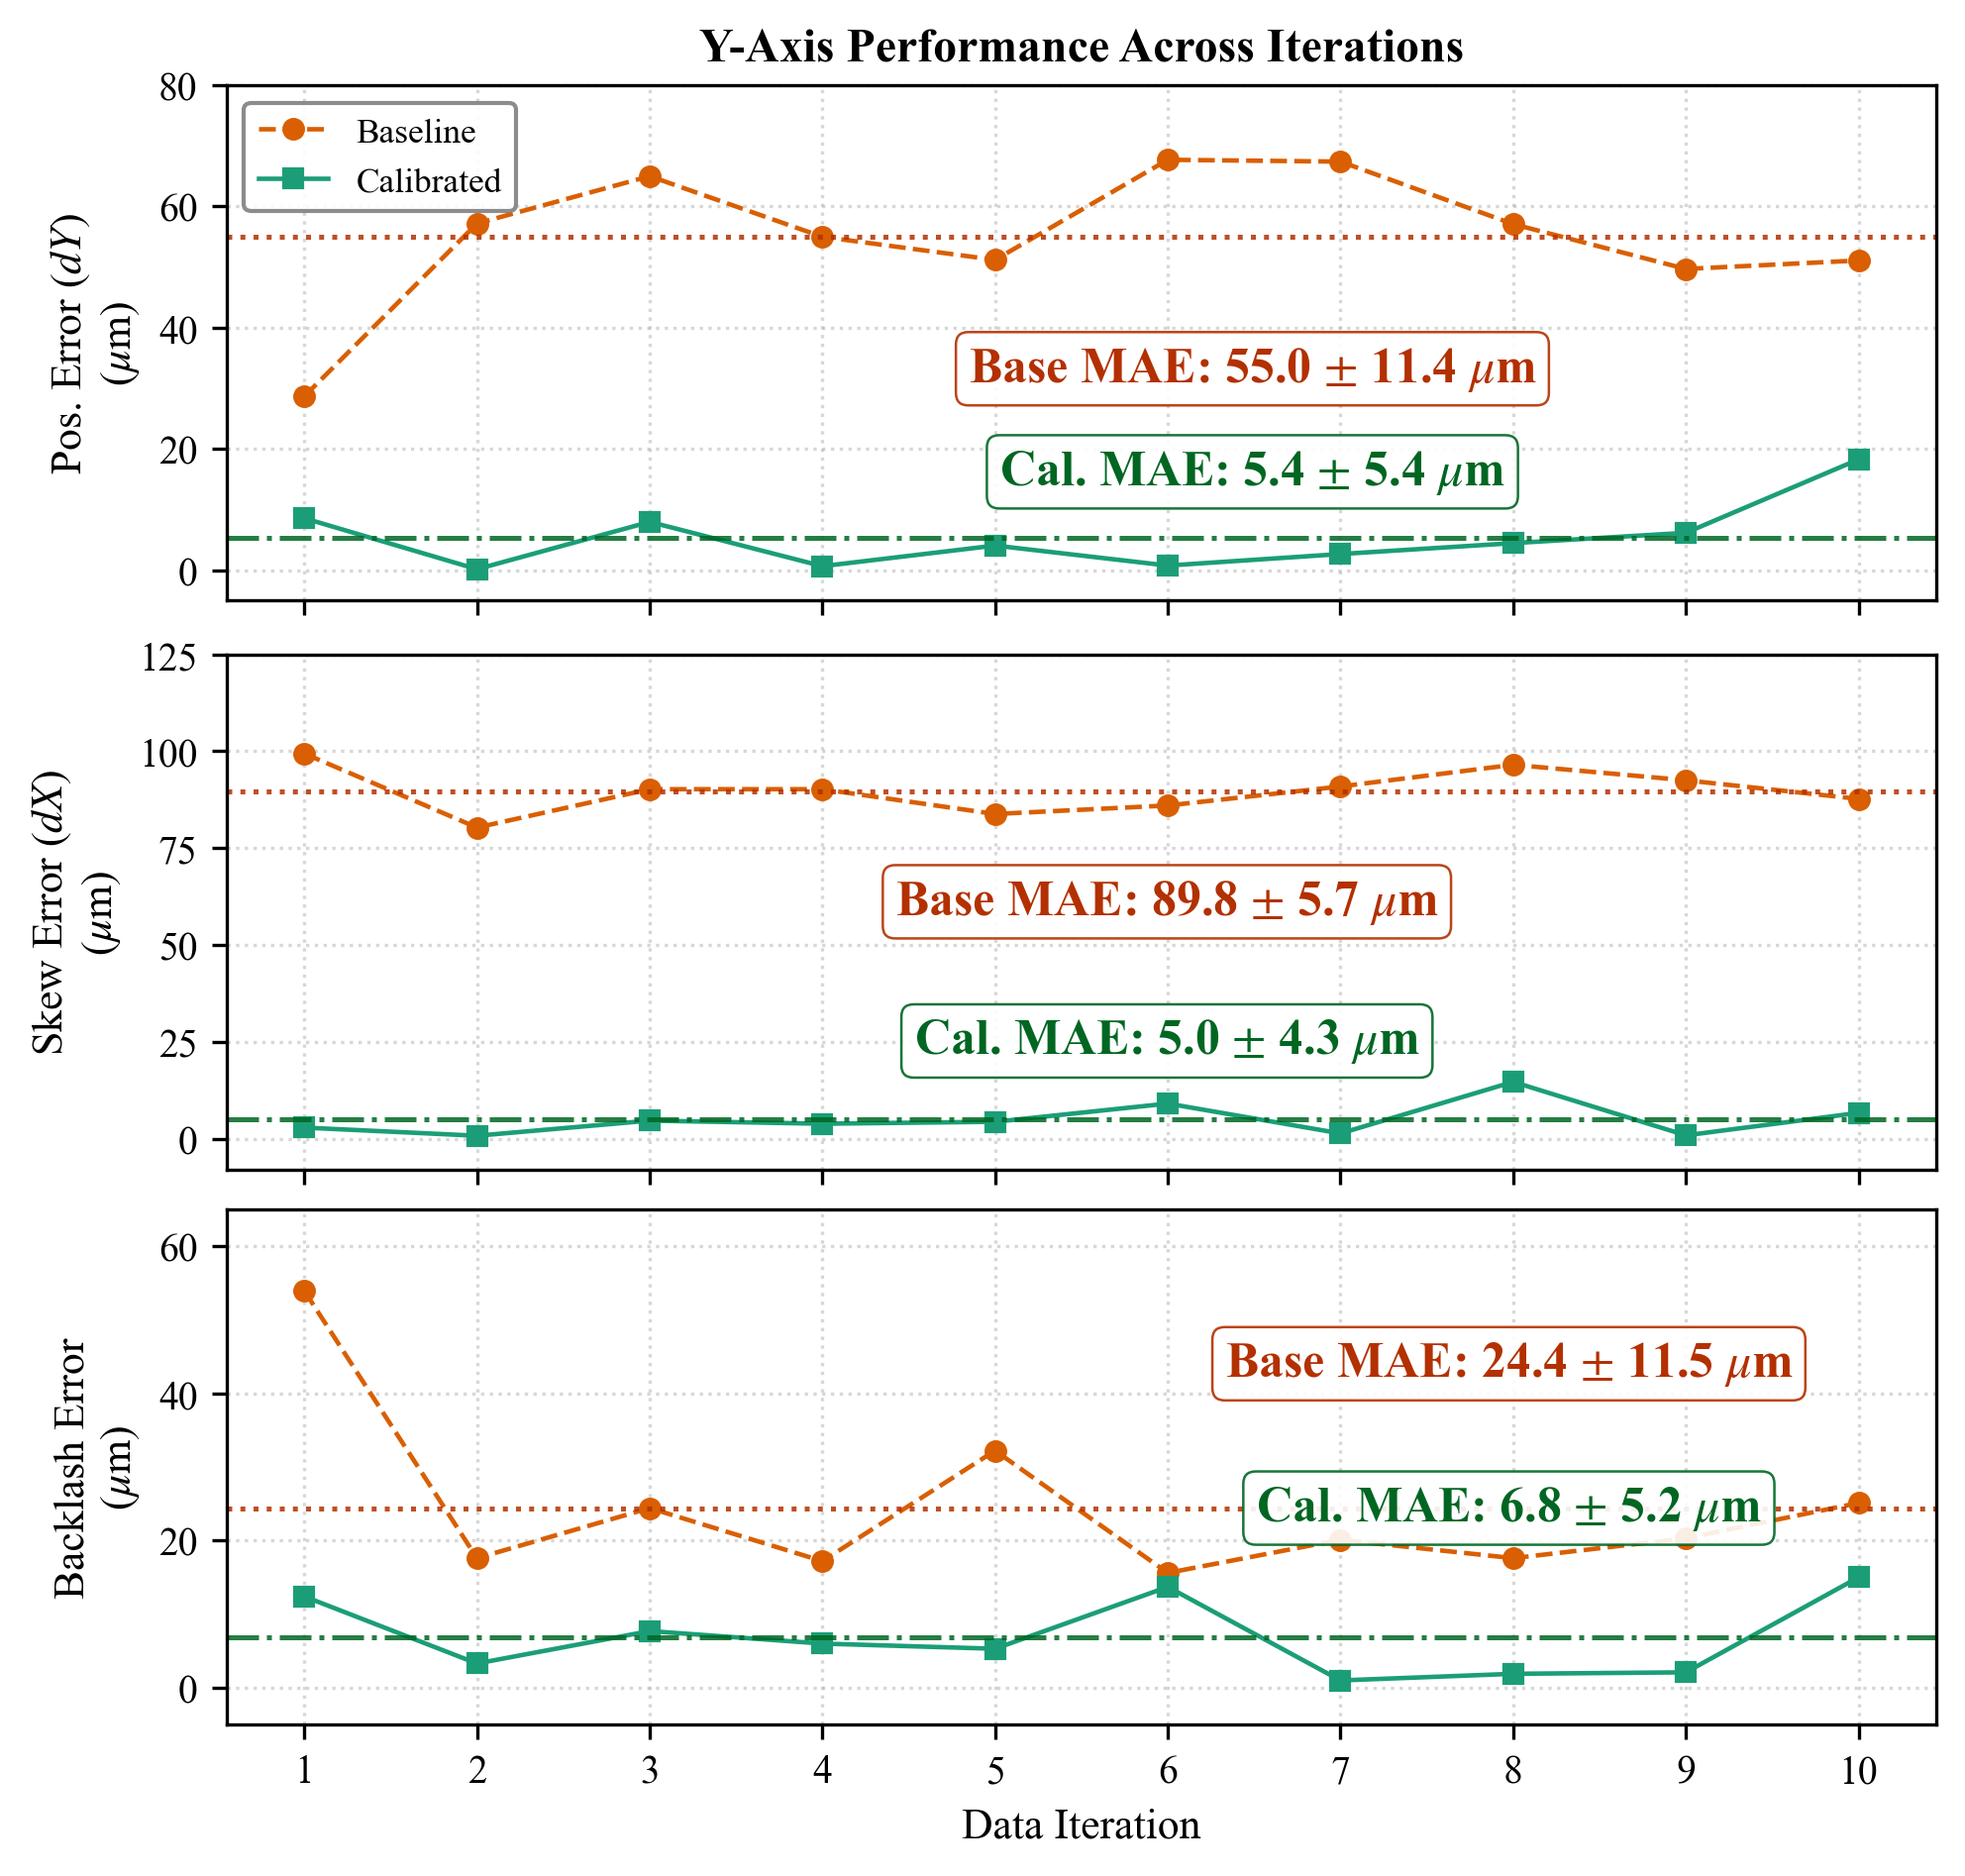
\includegraphics[width=1\linewidth]{images/y_axis_iterations.png}
	\caption{Y-axis single-axis error tracking across 10 iterations comparing baseline and calibrated states for positioning, skew, and backlash parameters.}
	\label{fig:y_axis_iter}
\end{figure}

Iterative fine-tuning systematically optimized the calibration constants over multiple correction cycles until a steady-state condition was reached. The final operational parameters converged at $79.72~\text{steps/mm}$ for the X-axis and $80.40~\text{steps/mm}$ for the Y-axis, with backlash compensations set to $13.3~\mu$m and $31.4~\mu$m, respectively. Cross-talk skew factors stabilized symmetrically at $\pm 9.2~\mu$m/mm. As shown in \figref{fig:maesum}, this optimization reduced linear axis errors to single-digit micrometers, matching the limits of the system's measurement resolution.

\begin{figure}[t]
	\centering
	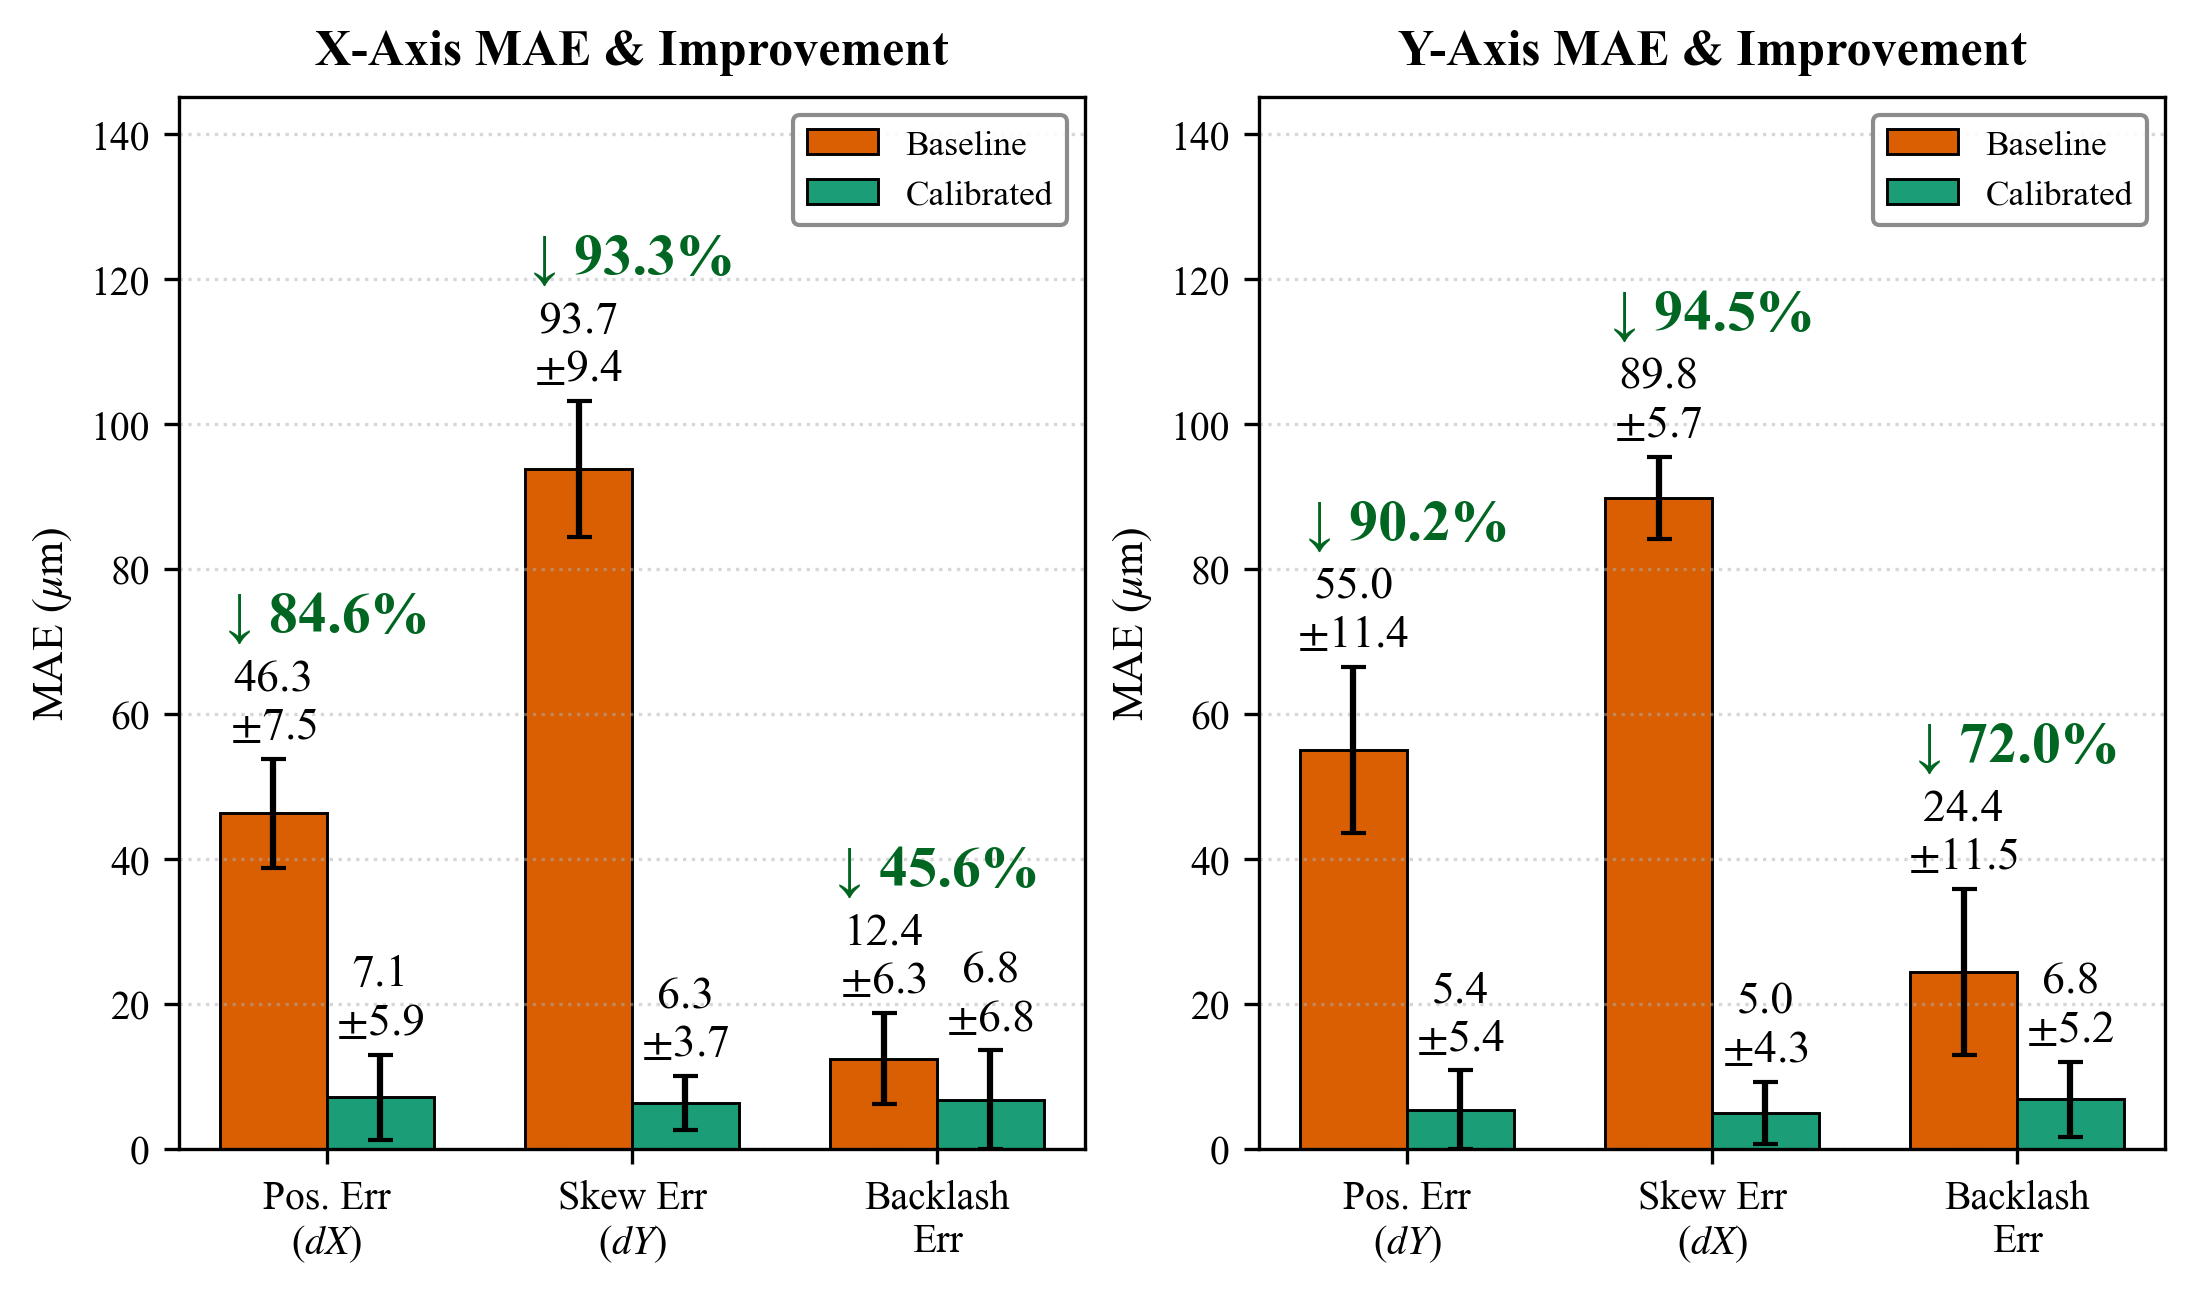
\includegraphics[width=1\linewidth]{images/mae_summary.png}
	\caption{Summary of Mean Absolute Errors (MAE) and percentage improvements across positioning, skew, and backlash metrics for X and Y axes.}
	\label{fig:maesum}
\end{figure}

\subsection{Simultaneous Trajectory Validation}
Dynamic tracking performance was evaluated by commanding the machine to trace a continuous elliptical trajectory, requiring synchronized, simultaneous motion across both axes. In the baseline state, the platform suffered from significant trajectory tracking deviations, resulting in an accumulated total Root Mean Square Error (RMSE) of $100.9 \pm 7.4~\mu$m.
Implementing the fine-tuned calibration parameters drastically corrected these trajectory deviations. The post-calibration X-axis tracking RMSE dropped to $34.42 \pm 1.70~\mu$m (a 55.25\% enhancement), while the Y-axis tracking RMSE was suppressed to $30.75 \pm 1.37~\mu$m (a 52.91\% enhancement). The total combined tracking error fell to $46.17 \pm 1.77~\mu$m, representing an overall trajectory accuracy improvement of 54.24\%. Visualization of the baseline performance and calibrated performance on one of the iterations while doing the trajectory movement shown in \figref{fig:vistrajectory}. The statistical result of the 10 iterations trajectory movement shown in \figref{fig:traj_rmse_iter} and \figref{fig:traj_summary_bars}.

\begin{figure}[!htbp]
	\centering
	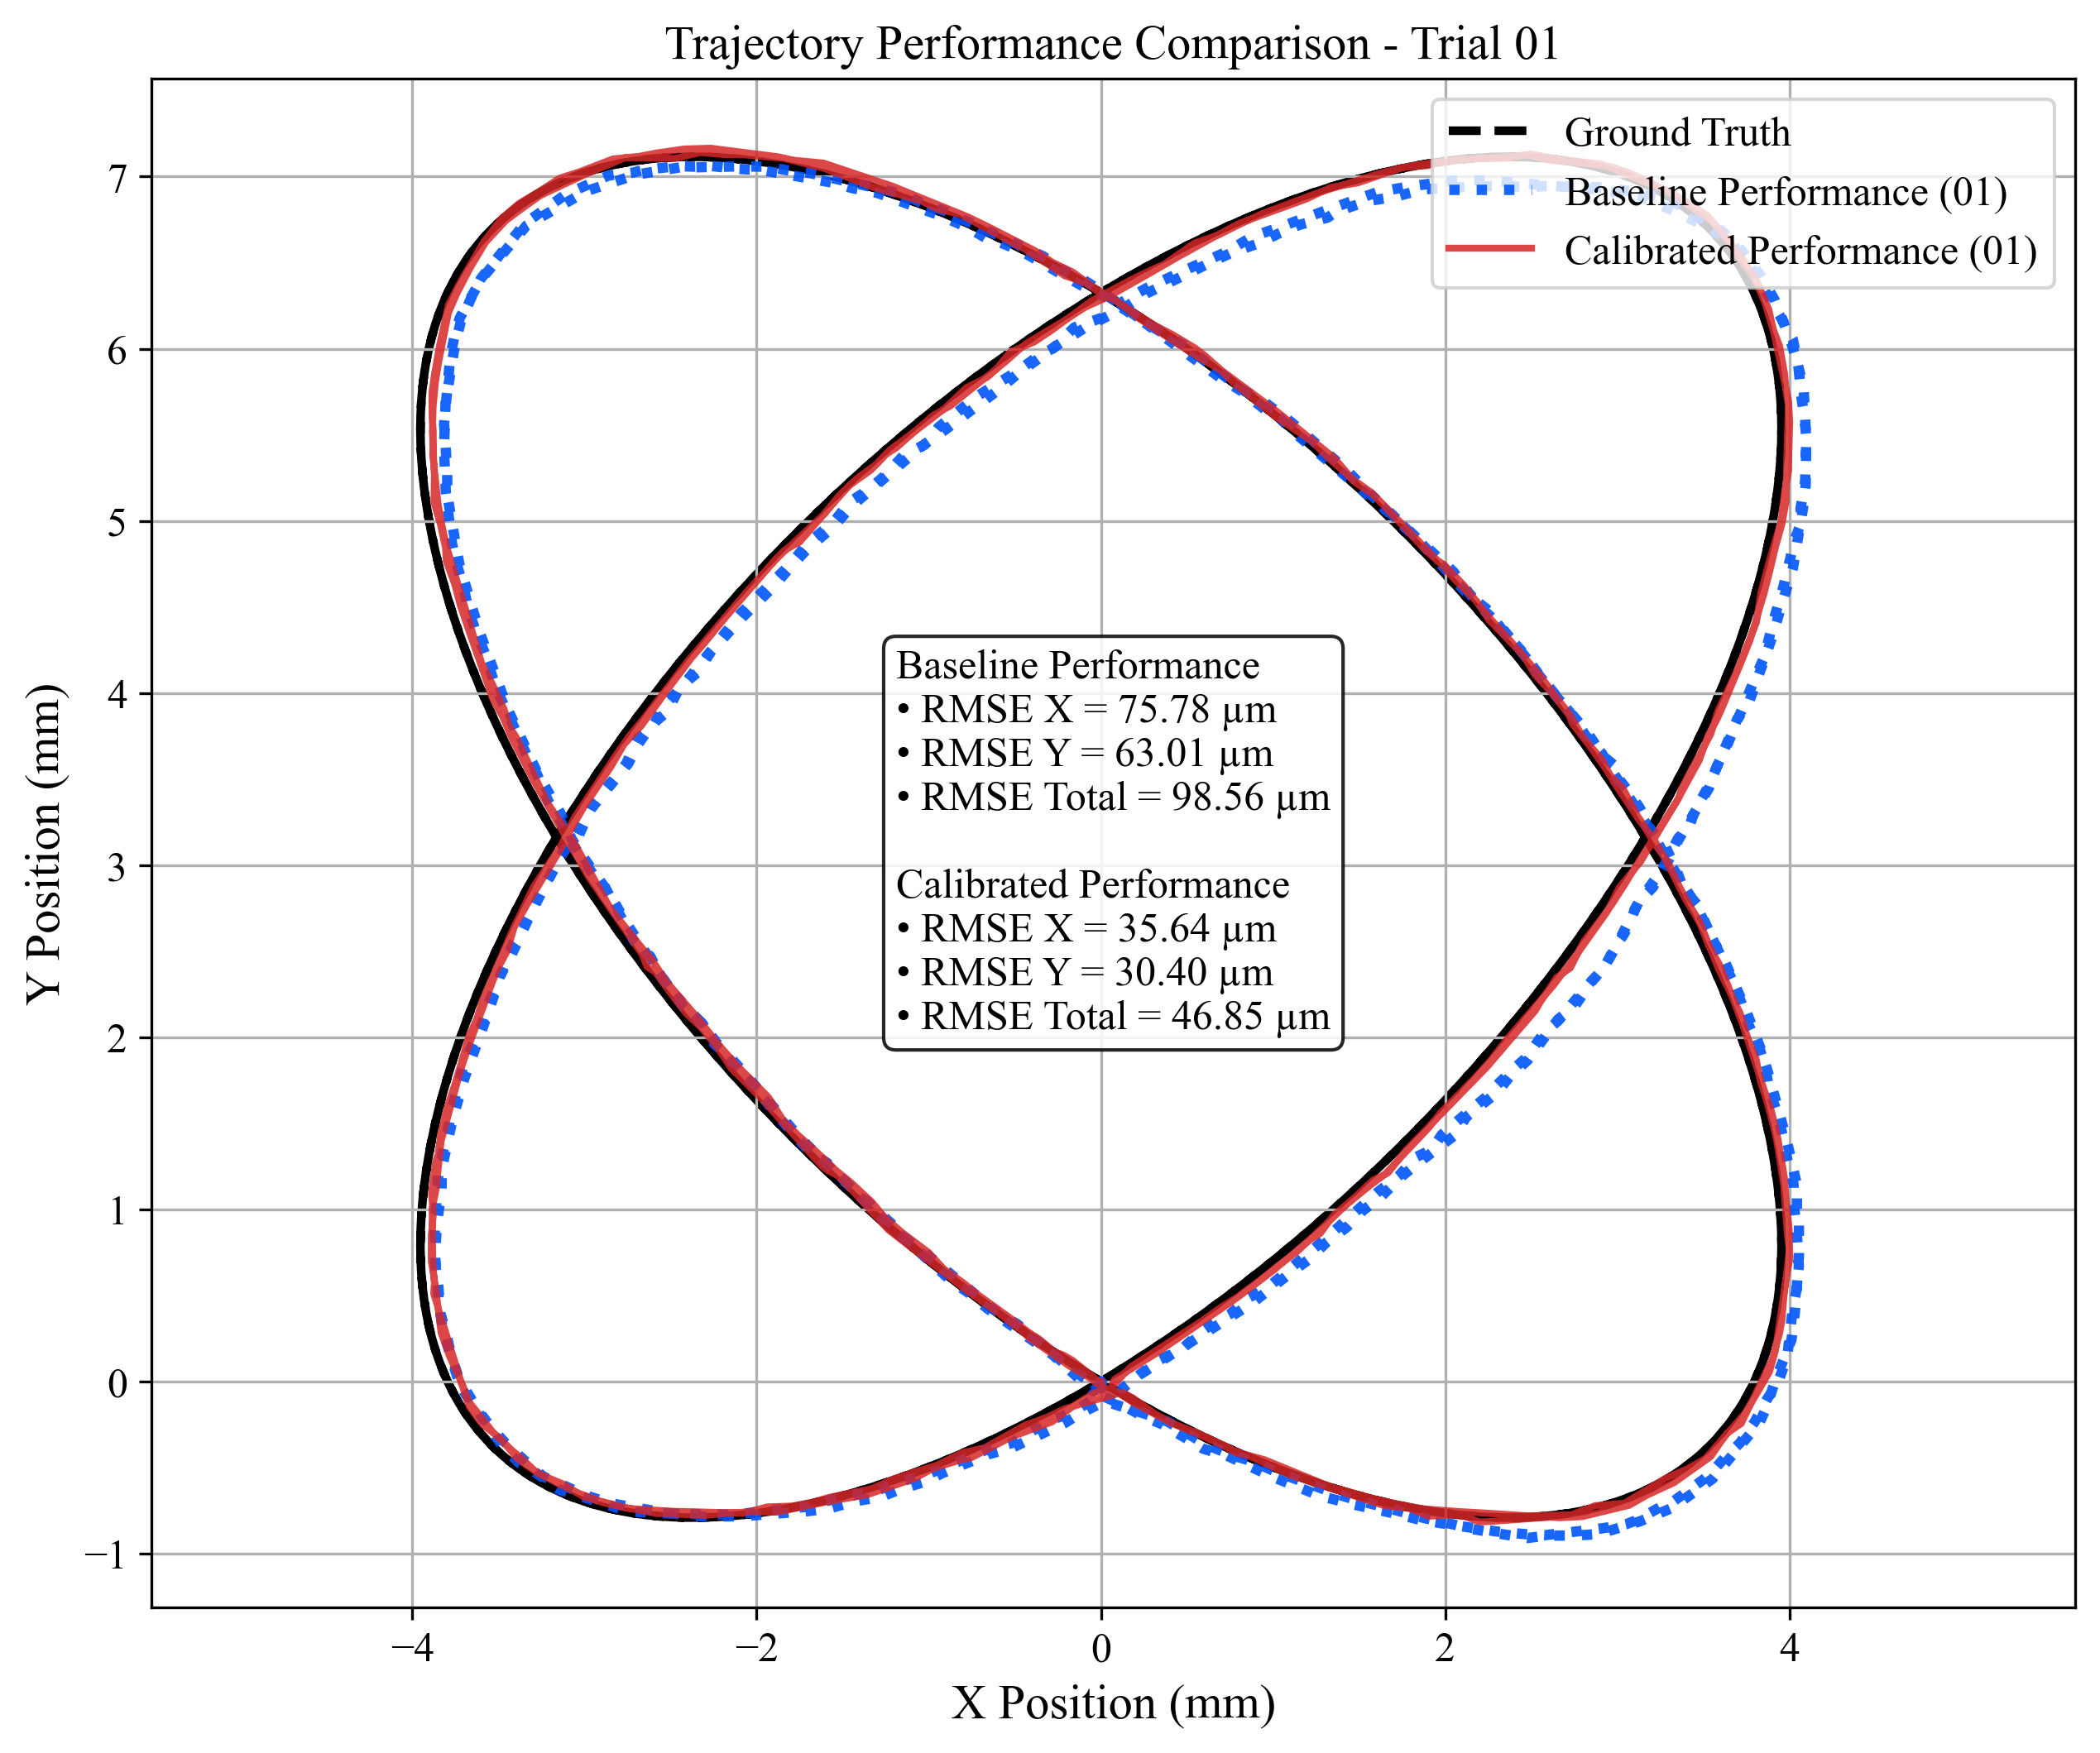
\includegraphics[width=1\linewidth]{images/perbandingan_full_01.png}
	\caption{Visualization of trajectory movement on baseline performance and calibrated performance.}
	\label{fig:vistrajectory}
\end{figure}

\begin{figure}[!htbp]
	\centering
	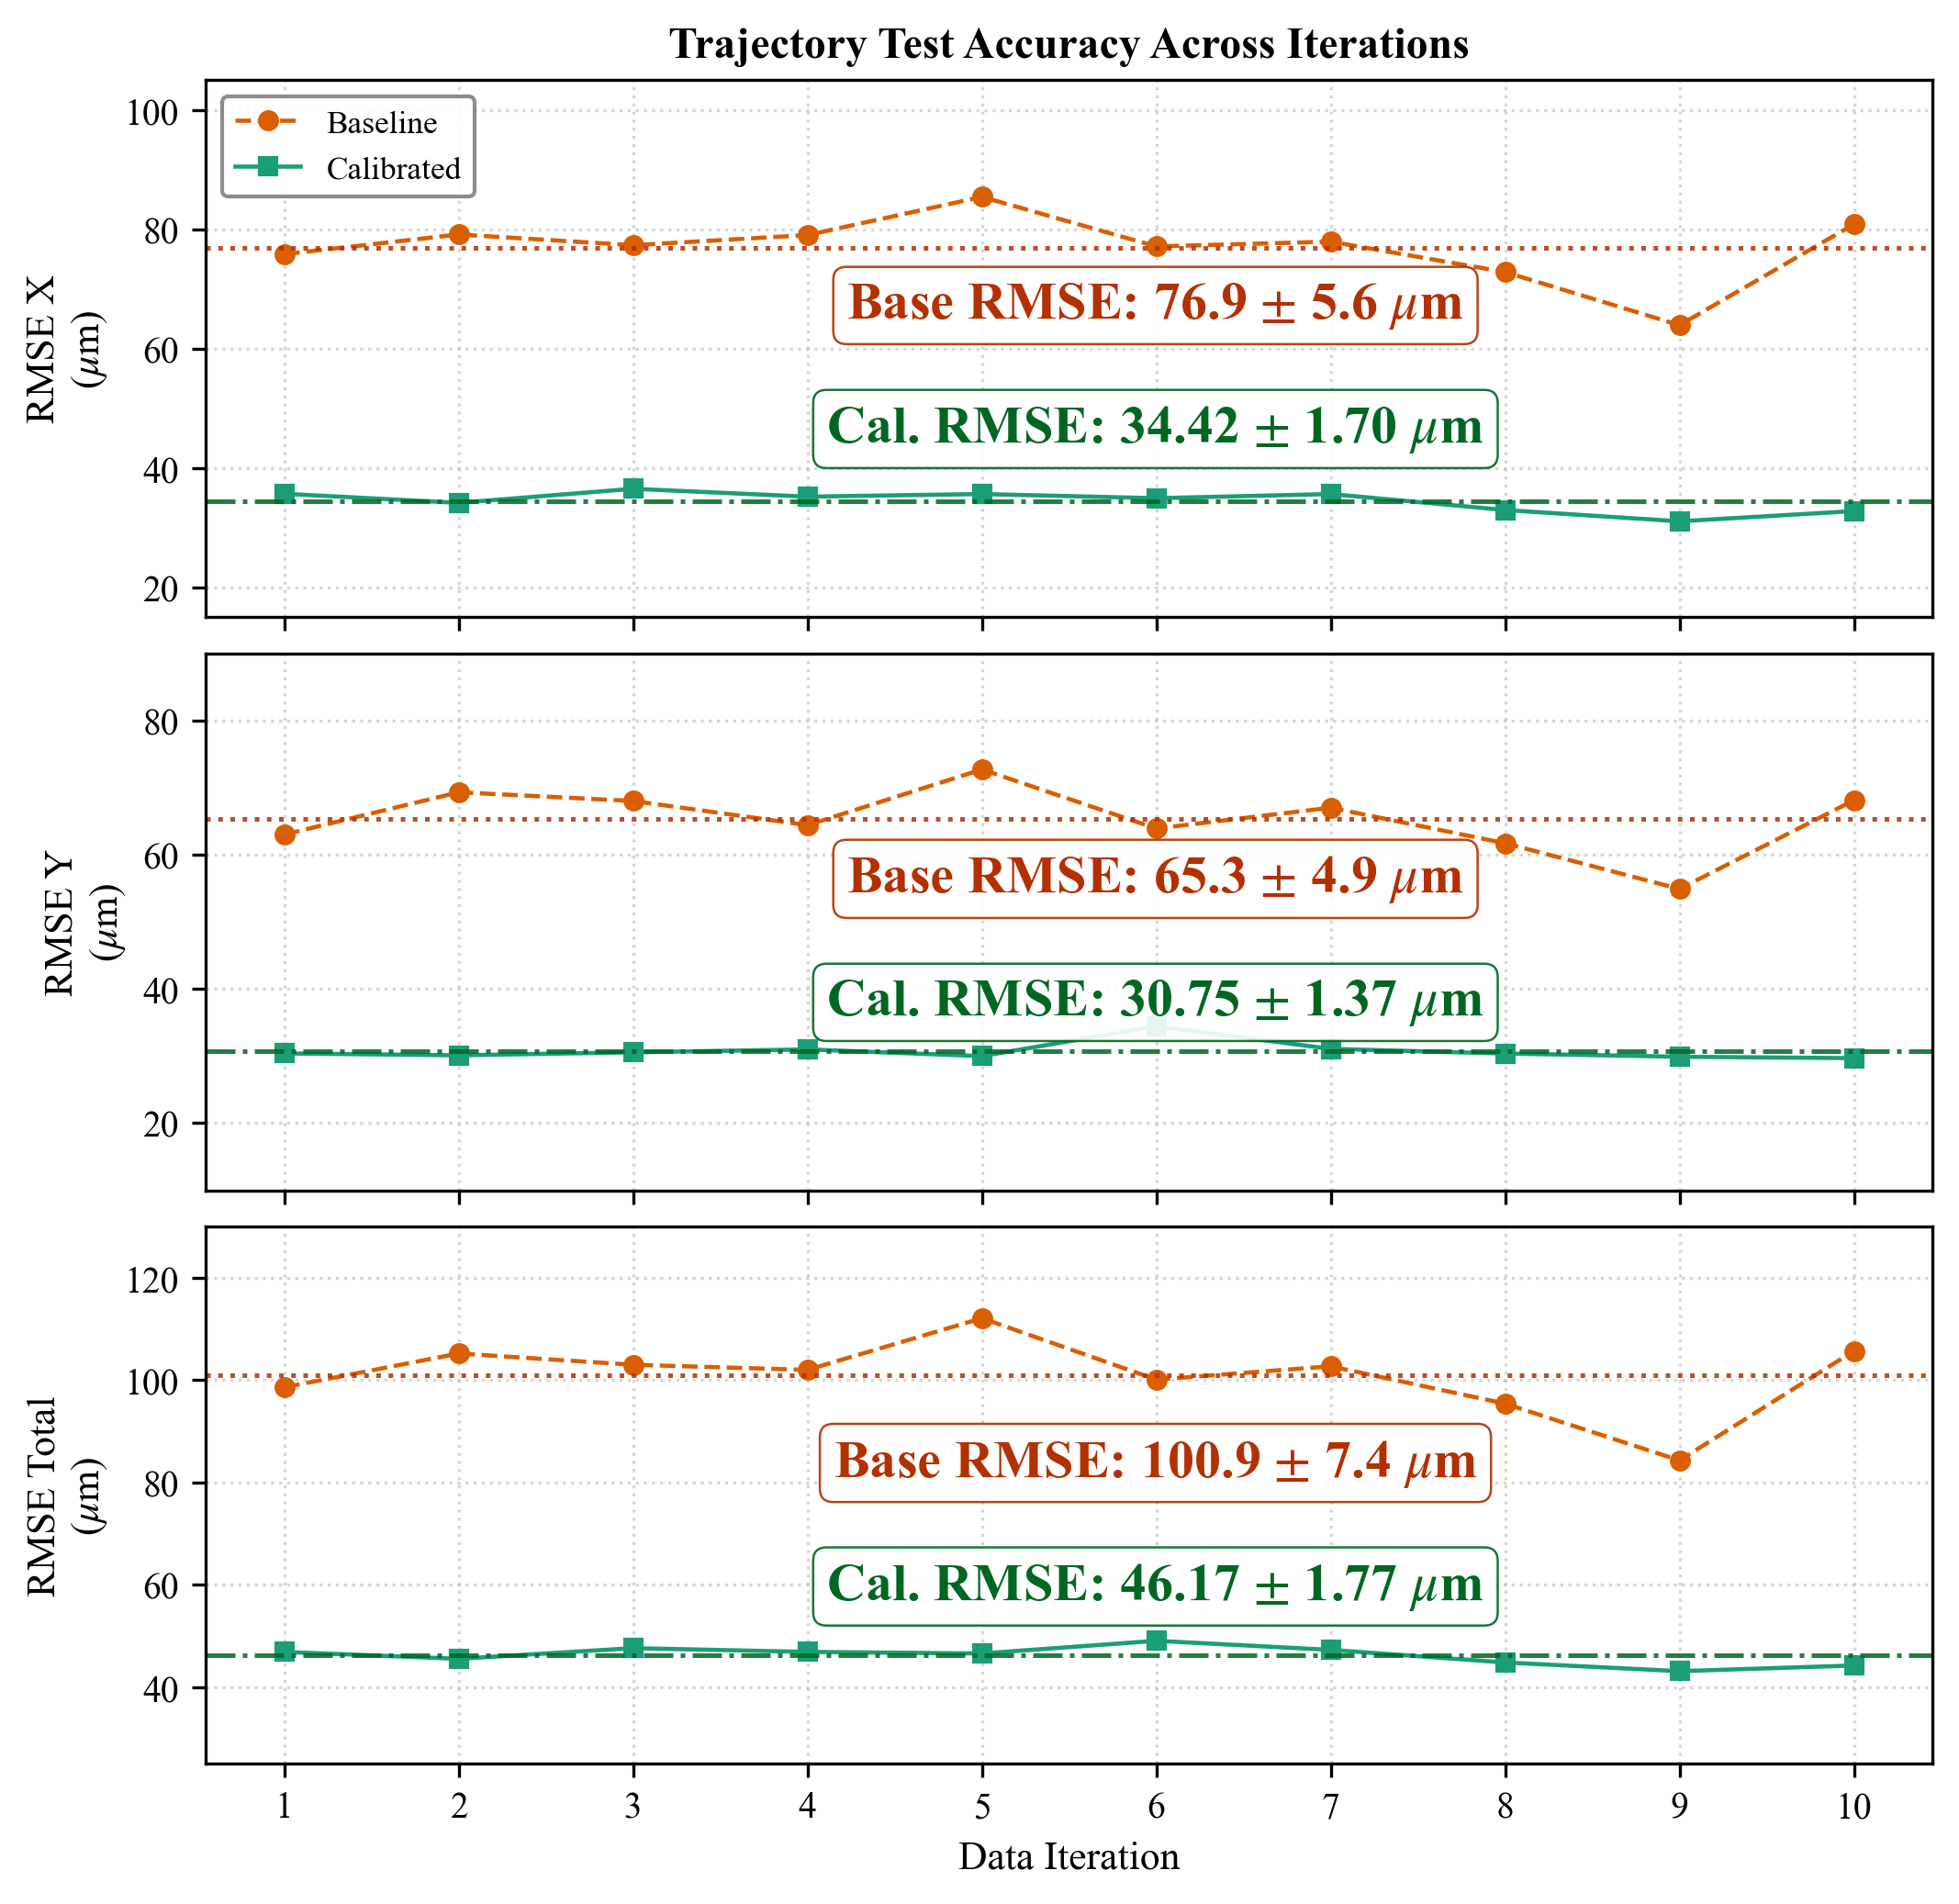
\includegraphics[width=1\linewidth]{images/trajectory_rmse_iterations_final.png}
	\caption{Tracking Root Mean Square Error (RMSE) across 10 iterations during continuous trajectory testing for X-axis, Y-axis, and total vector components.}
	\label{fig:traj_rmse_iter}
\end{figure}

\begin{figure}[!htbp]
	\centering
	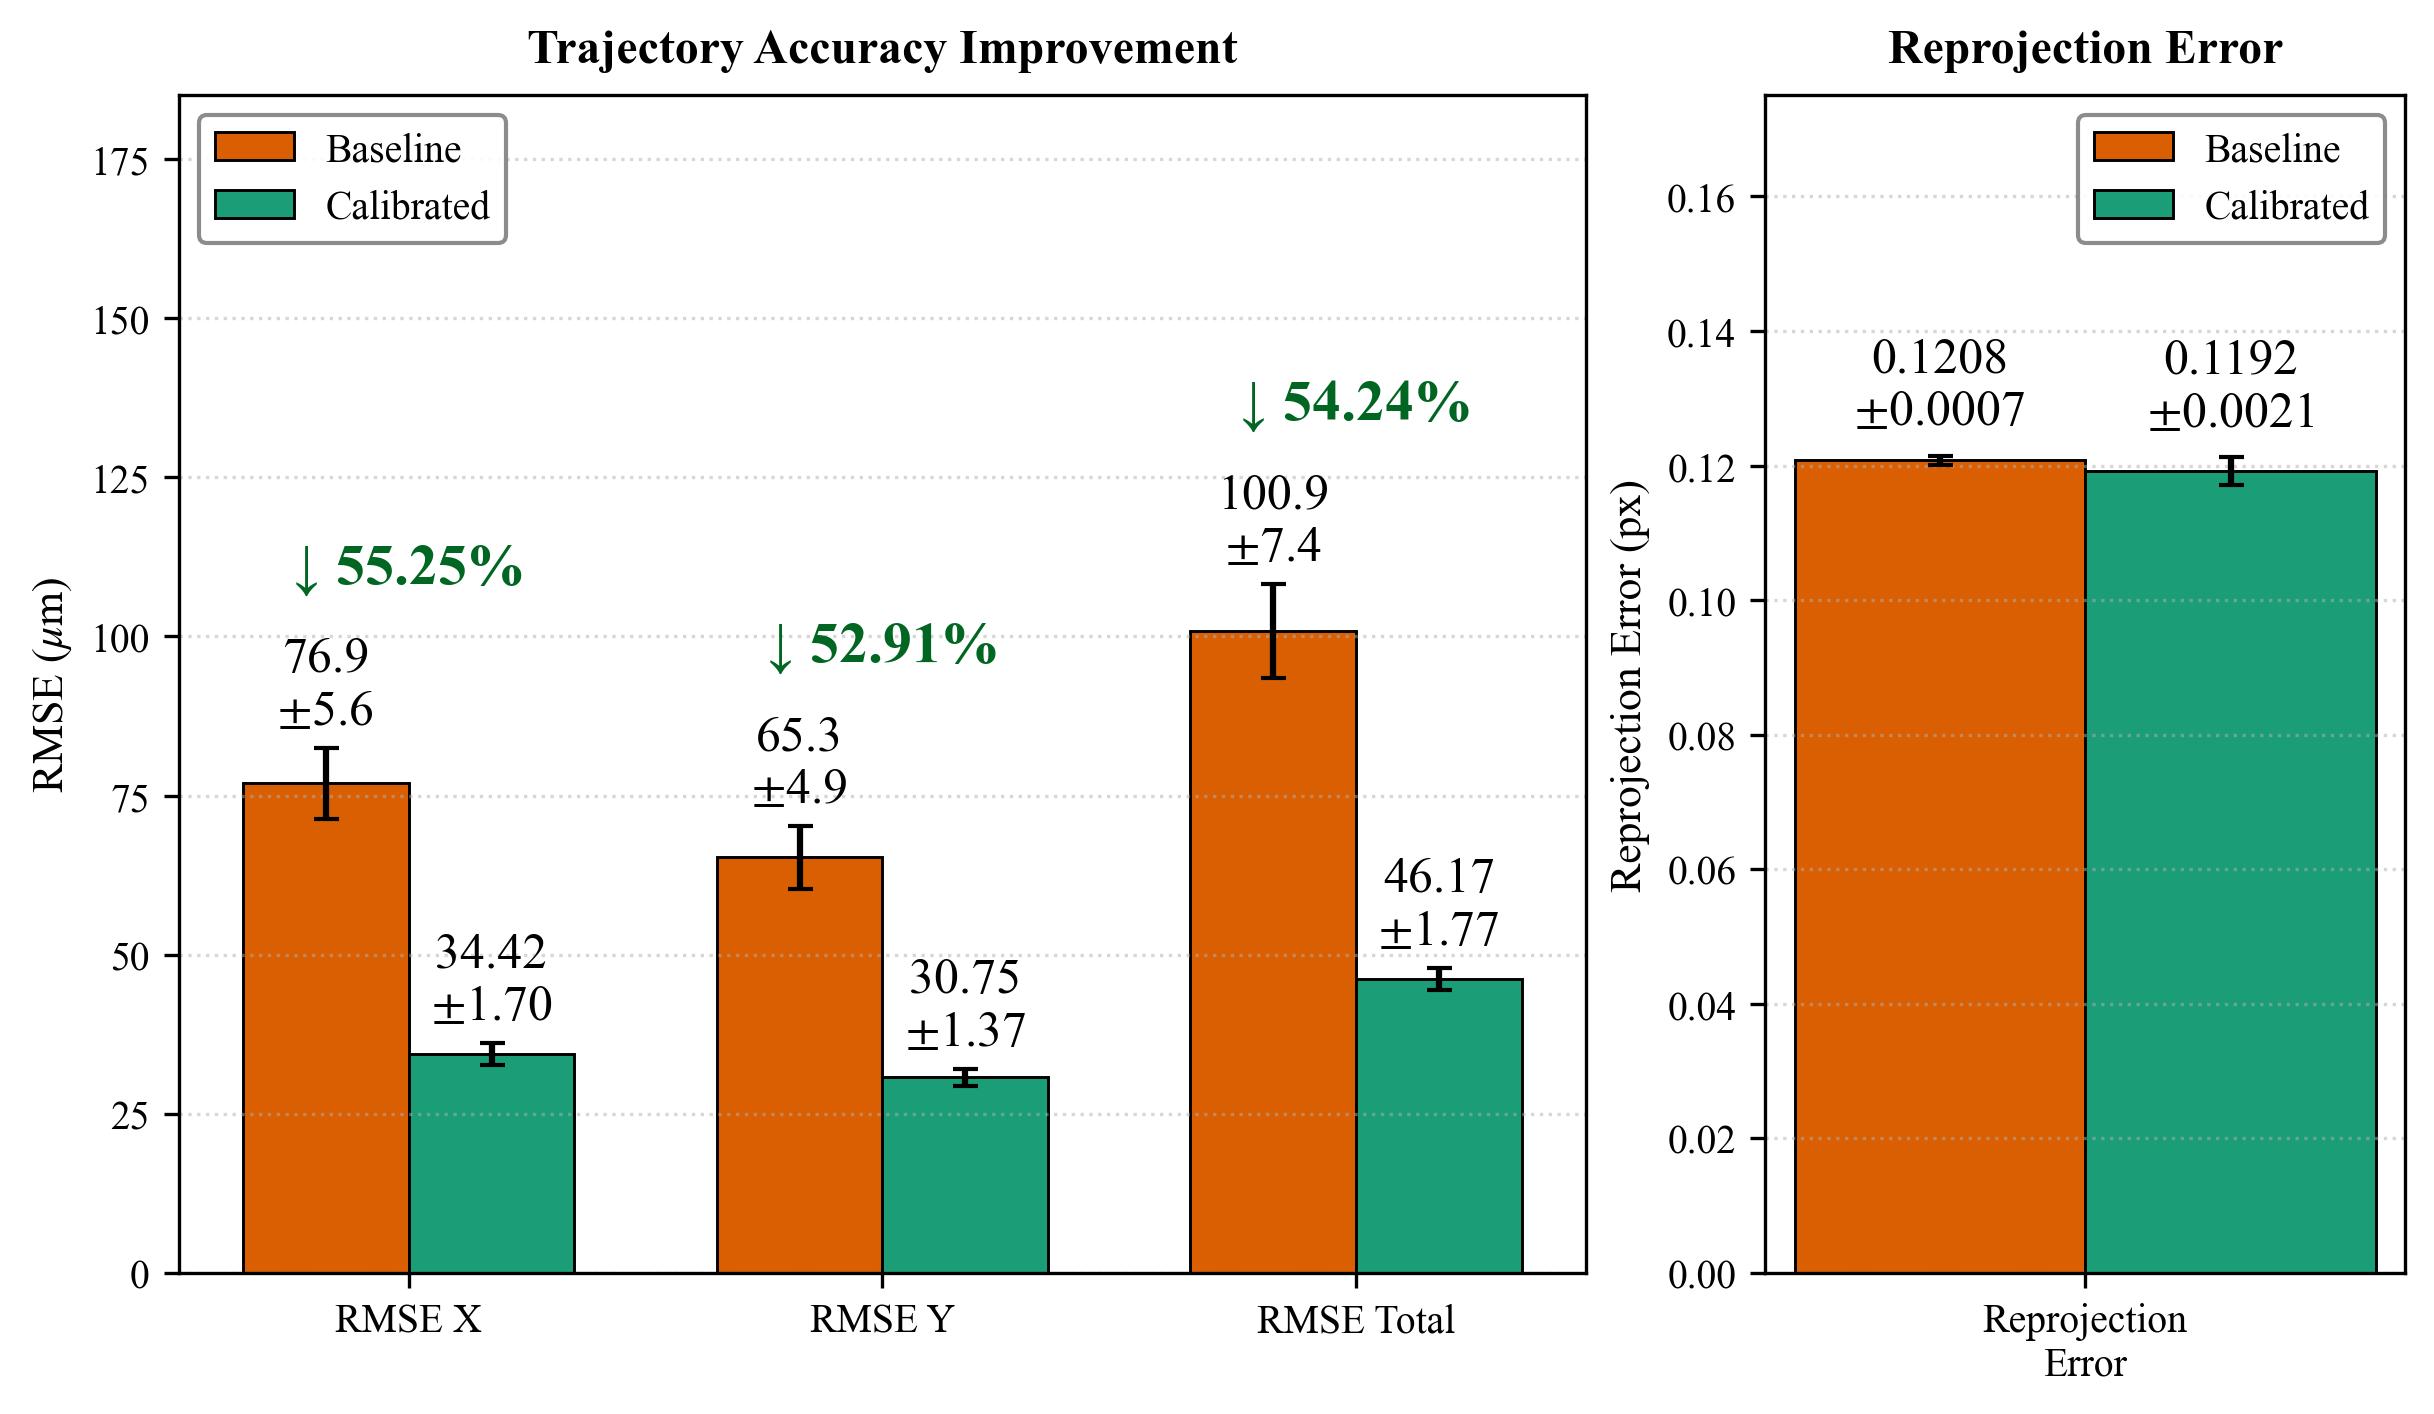
\includegraphics[width=1\linewidth]{images/trajectory_summary_bars_final.png}
	\caption{Statistical comparison of trajectory tracking accuracy improvements (RMSE X, Y, and Total) and reprojection error between baseline and calibrated system states.}
	\label{fig:traj_summary_bars}
\end{figure}

\subsection{Comparative Literature Analysis}
To evaluate commercial and scientific feasibility, the proposed virtual encoder was benchmarked against existing 3D printer calibration and kinematic measurement methodologies. Table~\ref{tab:literature_comparison} outlines the methodology performance, hardware requirements, and economic trade-offs across different approaches.

\providecommand{\newcolumntype}[2]{}
\newcolumntype{L}{>{\raggedright\arraybackslash}X}

\begin{table*}[ht]
	\centering
	\caption{Comparative Analysis of Calibration and Vision-Based Measurement Systems in Additive Manufacturing}
	\label{tab:literature_comparison}
	\scriptsize
	\setlength{\tabcolsep}{3pt}
	\renewcommand{\arraystretch}{1.2}
	
	\begin{tabularx}{\textwidth}{@{} L L L L L L @{}}
		\toprule
		\textbf{Category / Metric} & \textbf{Virtual Encoder (Proposed)} & \textbf{Owais et al. (2026) \cite{Owais2026}} & \textbf{Schouten et al. (2022) \cite{Schouten2022}} & \textbf{Chen \& Cai (2025) \cite{Chen2025}} & \textbf{Munteanu et al. (2021) \cite{Munteanu2021}} \\
		\midrule
		
		\textbf{Primary Domain} & 
		FDM Spatial Calibration \& Trajectory Tracking & 
		Spatial Vision Metrology \& Distortion & 
		Multi-Material Nozzle Offset Alignment & 
		Dual-Nozzle Spatial Auto-Calibration & 
		FDM Kinematic Error \& Trajectory Analysis \\
		
		\midrule
		\multicolumn{6}{@{}l}{\textbf{1. METHODOLOGY PERFORMANCE}} \\
		\midrule
		
		$\bullet$ \textbf{Measurement Error} & 
		$< 7~\mu\text{m} \mid 0.11\text{ px}$ & 
		$84~\mu\text{m} \mid 0.55\text{ px}$ & 
		$\approx 45~\mu\text{m}$ (Inductive vs. Optical) & 
		$< 100~\mu\text{m}$ ($0.1\text{ mm}$) & 
		Micron-level (Sensor resolution dependent) \\
		
		$\bullet$ \textbf{Positioning / Calibration} & 
		$8.92 \pm 5.42~\mu\text{m}$ & 
		$100 \pm 80~\mu\text{m}$ (Target region) & 
		$2~\mu\text{m}$ Inductive Repeatability & 
		$< 100~\mu\text{m}$ Nozzle Alignment & 
		$10 - 50~\mu\text{m}$ (Kinematic backlash / hysteresis) \\
		
		$\bullet$ \textbf{Dynamic Trajectory Tracking} & 
		Supported ($46.17 \pm 1.77~\mu\text{m}$ RMSE) & 
		N/A (Printed artifact: $30 \pm 20~\mu\text{m}$) & 
		N/A (Discrete Point Sensing) & 
		N/A (Static Nozzle Alignment) & 
		Supported (2D circular trajectory sampling) \\
		
		\midrule
		\multicolumn{6}{@{}l}{\textbf{2. HARDWARE REQUIREMENT}} \\
		\midrule
		
		$\bullet$ \textbf{Sensor / Camera Setup} & 
		1$\times$ Standard USB Monocular Camera & 
		Multi-Camera Rig (Stereo / Multi-view) & 
		Bed-Integrated Coil + A4 Scanner & 
		1$\times$ Internal Monocular Camera & 
		2$\times$ Non-Contact Optical Sensors \\
		
		$\bullet$ \textbf{Target / Physical Fixture} & 
		Planar Chessboard Target on Toolhead & 
		Volumetric Calibration Rig \& Artifacts & 
		Conductive Metallic Nozzle (Mandatory) & 
		Bed-Mounted Optical Prism \& LED Module & 
		External Calibration Reference Fixture \\
		
		$\bullet$ \textbf{Computing Infrastructure} & 
		External Host PC \& Standard MCU (Marlin) & 
		Vision Metrology Workstation & 
		Embedded MCU + PC Image Processing & 
		Integrated Compute Module / Host PC & 
		External DAQ System \& Computer Processing \\ 
		
		\midrule
		\multicolumn{6}{@{}l}{\textbf{3. ECONOMIC TRADE-OFFS}} \\
		\midrule
		
		$\bullet$ \textbf{Module Hardware Cost} & 
		Low ($\sim\$10 - \$25$) & 
		Medium -- High (Multi-camera rig) & 
		Very Low (PCB coil) / Scanner extra & 
		Low -- Medium (Standard camera) & 
		Medium -- High (Specialized optical sensors) \\
		
		$\bullet$ \textbf{MCU Computational Load} & 
		None (Offloaded to Host PC) & 
		Heavy (Offline multi-view processing) & 
		Very Light (Real-time inductance) & 
		Medium (Hough/Color Segmentation) & 
		None (External DAQ system processing) \\
		
		$\bullet$ \textbf{Implementation Complexity} & 
		Low -- Medium (Monocular \& planar target) & 
		High (Multi-camera stereo alignment) & 
		Medium (Print bed modification) & 
		Low (Bed-mounted prism \& camera setup) & 
		Medium (Rigid sensor mounting \& alignment) \\
		
		$\bullet$ \textbf{Automation \& Efficiency} & 
		Automated Data Acquisition and Offline Frame Analysis & 
		Offline Metrology Mapping & 
		Automated (Inductive) / Manual (Paper) & 
		Automated (Pre-print routine) & 
		Offline Trajectory Signal Analysis \\
		
		\bottomrule
	\end{tabularx}
\end{table*}
\section{Conclusion and Future Work}
\label{conclusion}
This study presented a low-cost, machine vision-based virtual encoder for 3D printer kinematic calibration, integrating a planar chessboard marker, an EDLines extraction pipeline, and an iterative SolvePnP solver. Characterization testing established a mean reprojection error of $0.1192 \pm 0.0021\text{ px}$, an internal static noise floor of $2.58~\mu\text{m}$ ($\sigma = 2.5~\mu\text{m}$) on the X-axis and $4.9~\mu\text{m}$ ($\sigma = 3.3~\mu\text{m}$) on the Y-axis, and absolute measurement errors of $3.55~\mu\text{m}$ and $6.25~\mu\text{m}$, respectively. Following fine-tuning, the calibration framework systematically mitigated all linear error components: X-axis positioning, skew, and backlash errors were reduced by 84.6\% (to $7.1 \pm 5.9~\mu\text{m}$), 93.3\% (to $6.3 \pm 3.7~\mu\text{m}$), and 45.6\% (to $6.8 \pm 6.8~\mu\text{m}$), while Y-axis metrics decreased by 90.2\% (to $5.4 \pm 5.4~\mu\text{m}$), 94.5\% (to $5.0 \pm 4.3~\mu\text{m}$), and 72.0\% (to $6.8 \pm 5.2~\mu\text{m}$). Furthermore, dynamic trajectory tracking error was suppressed by 54.24\%, yielding a total path RMSE of $46.17 \pm 1.77~\mu\text{m}$. These empirical findings confirm that software-driven error compensation effectively resolves multi-axis mechanical imperfections under a hardware budget below 30 USD. 

Future work will focus on integrating telecentric optics to minimize perspective distortion and developing a rigid, CNC-machined enclosure mounted on a modular toolhead to reduce structural flexing during dynamic calibration.

% --- BIBLIOGRAPHY ---
\bibliographystyle{IEEEtran}
\bibliography{IEEEabrv,Bibliography}

\end{document}